% =====================================================================
%   AgentBench: Evaluating LLMs as Agents  (Chinese Translation)
%   Compile with:   xelatex main.tex   (two passes recommended)
% =====================================================================
\documentclass[11pt,a4paper]{article}

% ---------- 中文支持（ctex：自动选用系统中文字体） ----------
\usepackage[UTF8,fontset=none,space=auto]{ctex}
% 说明：
%   - fontset=none 关闭 ctex 自带的默认字体集，改为下面手工指定，避免硬编码
%     Windows 字体，在 Linux/macOS 上也仍能正常编译。
%   - space=auto    让 ctex 自动在中英文之间加入合理空格。

% ---------- 数学 / 符号 ----------
\usepackage{amsmath,amssymb,amsfonts}

% ---------- 图形与表格 ----------
\usepackage{graphicx}
\usepackage{booktabs,tabularx,multirow,multicol}
\usepackage{array}

% ---------- 链接 / 颜色 ----------
\usepackage{hyperref}
\hypersetup{
    colorlinks=true,
    linkcolor=blue!60!black,
    citecolor=teal!70!black,
    urlcolor=blue!70!black,
    pdftitle={AgentBench: Evaluating LLMs as Agents (中文翻译)},
    pdfauthor={Xiao Liu 等 / 译注版}
}
\usepackage{xcolor}
\usepackage[round]{natbib}        % 提供 \citep / \citet 等
\bibliographystyle{plainnat}      % 在 references.tex 中已直接采用 thebibliography

% ---------- 页面设置 ----------
\usepackage{geometry}
\geometry{a4paper,left=2cm,right=2cm,top=2.5cm,bottom=2.5cm,headheight=14pt}

% ---------- 中文字体手工指定（兼容多平台） ----------
%   ctex 在 fontset=none 时由 xeCJK 接管，我们用字体名称族切换
\setCJKmainfont[BoldFont={SimHei},ItalicFont={KaiTi}]{SimSun}
\setCJKsansfont{SimHei}
\setCJKmonofont{FangSong}
% 西文沿用默认 Computer Modern 即可（避免与中文字体名称冲突）

% ---------- 行距 / 段距 ----------
\linespread{1.25}
\setlength{\parskip}{0.4\baselineskip}
\setlength{\parindent}{2em}

% ---------- 图形搜索路径 ----------
\graphicspath{{./}{./figures/}{../figures/}{figures/}}

% ---------- 定理 / 定义环境（来自 amsthm） ----------
\usepackage{amsthm}
\newtheorem{definition}{定义}
\newtheorem{theorem}{定理}
\newtheorem{proposition}{命题}
\newtheorem{lemma}{引理}
\theoremstyle{definition}
\newtheorem{example}{示例}

% ---------- 中文图 / 表 / 算法标题格式 ----------
% （已在 preamble 中预留 caption 配置位，以下行为空，移除之避免重定义）


% ---------- 列表 / 引用 / 其它辅助包 ----------
\usepackage{enumitem}
\setlist[itemize]{leftmargin=*,topsep=2pt,itemsep=1pt}
\usepackage{footmisc}
\renewcommand{\thefootnote}{\arabic{footnote}}

% ---------- 算法环境（附录多处用）----------
\usepackage{algorithm}
\usepackage{algorithmic}

% ---------- 同一行内联代码、键入样式 ----------
%   普通 \texttt 会将 '_' 解析为下标；这里使用 \nolinkurl 等价方式
%   （由 hyperref 提供），安全显示 _、&、% 等字符
\newcommand{\code}[1]{\texttt{\detokenize{#1}}}

% ---------- 双语标题宏（少数专有名词用） ----------
\newcommand{\EN}[1]{\emph{#1}}

% ---------- 章节标题微调（贴近原文 ICLR 论文排版） ----------
\usepackage{titlesec}
\titleformat*{\section}{\large\bfseries}
\titleformat*{\subsection}{\normalsize\bfseries}
\titleformat*{\subsubsection}{\normalsize\bfseries}

% ---------- 中文图 / 表 / 算法标题格式 ----------
\usepackage{caption}
\captionsetup{font=small,labelsep=quad,labelfont={bf}}
\captionsetup[table]{skip=4pt}

% =====================================================================
\title{\vspace{-1.0cm}\textbf{AgentBench：将大语言模型作为智能体进行评估}\\
\large 原论文中文翻译稿\\(ICLR 2024)}
\author{原\ 作：Xiao Liu, Hao Yu, Hanchen Zhang, Yifan Xu, Xuanyu Lei,
        Hanyu Lai, Yu Gu, Hangliang Ding, Kaiwen Men, Kejuan Yang,\\
        Shudan Zhang, Xiang Deng, Aohan Zeng, Zhengxiao Du, Chenhui Zhang,\\
        Sheng Shen, Tianjun Zhang, Yu Su, Huan Sun, Minlie Huang,\\
        Yuxiao Dong, Jie Tang\\[2pt]
        （清华大学\ \ The Ohio State University\ \ UC Berkeley）}
\date{}
% =====================================================================
\begin{document}
\maketitle

% 论文首页脚注式头注（原论文 ICLR 头注 + 中文致谢）
\begin{center}
\small
Published as a conference paper at ICLR 2024.\\
（原论文发表于 ICLR 2024。本文为其中文翻译稿，仅供学术交流使用。）
\end{center}

% 引入后文各章节
% =====================================================================
%   摘要 (Abstract)
% =====================================================================

\section*{摘\quad 要}

近年来，大语言模型（Large Language Model, LLM）作为智能体的潜力已被广泛认可。
因此，迫切需要在具有挑战性的交互式环境任务上，对将 LLM 作为智能体的能力
进行定量评估。本文提出 \textbf{AgentBench}——一个由 8 个不同环境组成的多维度
基准（benchmark），用以评估 LLM 作为智能体（LLM-as-Agent）的推理与决策能力。
我们在 29 个基于 API 的商用 LLM 与开源（Open-Sourced, OSS）LLM 上进行了大规模
测试，结果显示：尽管顶尖商用 LLM 在复杂环境中展现出强大的智能体行为能力，
但其与众多规模不超过 70B 的开源竞品之间仍存在显著的性能差距。
我们进一步识别了环境与 LLM 各自的典型失败原因，发现较弱的长期推理、决策与
指令遵循能力是当前阻碍 LLM 智能体走向实用化的主要瓶颈。提升指令遵循能力，
并在高质量多轮对齐数据上进行训练，可有效改进智能体表现。此外，与既有
认知不同，本文发现代码训练对不同智能体任务的影响具有两面性。

本文相关的数据集、环境与一体化评估包已发布于
\url{https://github.com/THUDM/AgentBench}。

\begin{figure}[t]
    \centering
    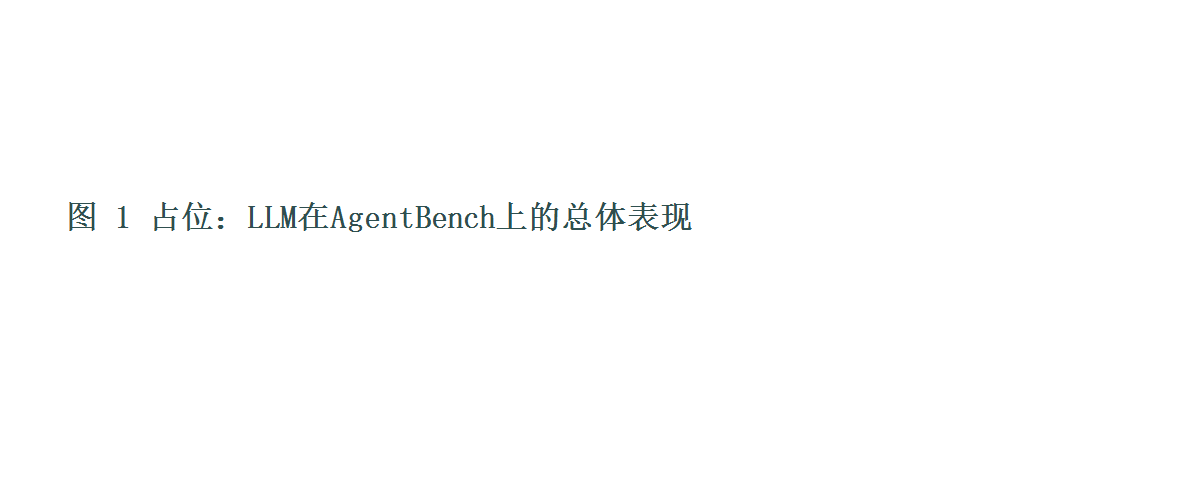
\includegraphics[width=0.85\linewidth]{overview_placeholder.png}
    \caption{
        本图为原论文图 1 的中文译图——\textbf{LLM 在 AgentBench 上的总体表现}。
        左侧将各环境下的典型 LLM 表现与最佳模型对齐显示；右侧给出 29 个
        LLM 在 8 个环境上的总体得分，虚线分别表示 API 类商用 LLM 与
        OSS LLM 的平均分。可以看出：商用 LLM 平均得分显著高于 OSS LLM，
        但即便是最强的 \code{gpt-4}，距离真正实用化的智能体仍有可观差距。
    }
    \label{fig:overview}
\end{figure}

% 注释：保持章节连续，自然从 \section{引言} 开始即可（见 intro.tex）。
% 本翻译稿中不再重置计数器，避免后续页被推到下一页。

% =====================================================================
%   1. 引言 (Introduction)
% =====================================================================

\section{引言}

能够在特定环境中进行决策与动作执行的智能体（intelligent agent）与自主实体
（autonomous entity）\citep{searle1970,maes1994,wooldridge1995}，自古以来都是人工智能
（Artificial Intelligence, AI）研究中的核心概念。尽管深度学习算法在计算机视觉与
自然语言处理（Natural Language Processing, NLP）领域已取得长足进展，但其用于开发
高效且实用的辅助型智能体的潜力，迄今仍未被充分挖掘。

\begin{figure}[t]
    \centering
    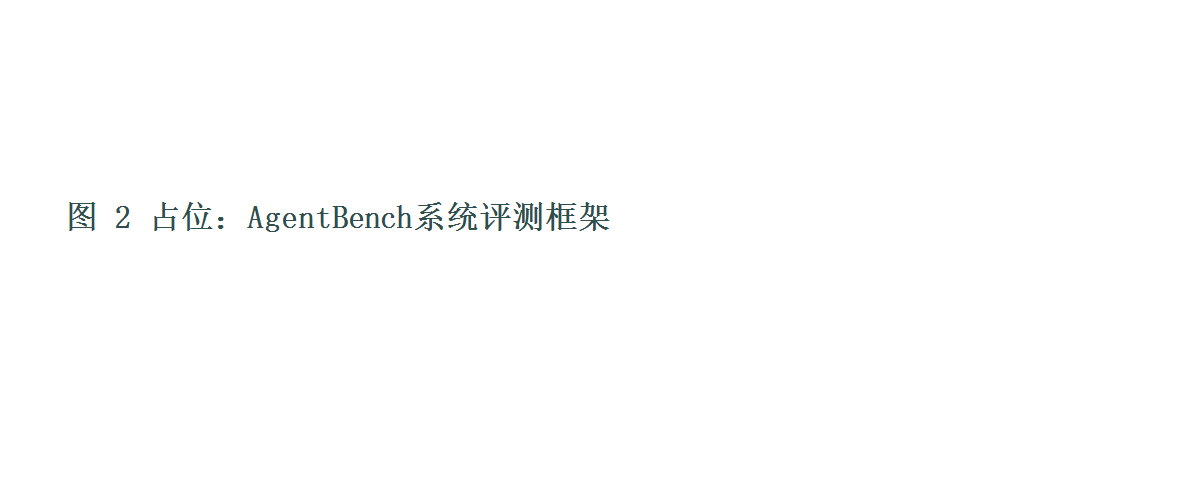
\includegraphics[width=0.95\linewidth]{realworld_placeholder.png}
    \caption{
        本图为原论文图 2 的中文译图——\textbf{AgentBench 在 8 类真实环境下的
        系统化评测框架}。左侧为现实世界中的典型挑战，右侧为 8 个面向不同
        真实场景的交互式环境，LLM 作为智能体居于其间，通过感知环境、下达
        动作与之交互。本文首版共评测了 29 个 LLM。
    }
    \label{fig:realworld}
\end{figure}

大语言模型（Large Language Model, LLM）的兴起
\citep{brown2020,chowdhery2022,touvron2023}，以 \code{GPT-4} \citep{openai2023} 为代表，
为这一研究领域注入了崭新的机遇。通过大量对齐训练
\citep{ouyang2022,wei2022a,sanh2022}，LLM 不仅熟练掌握了传统 NLP 任务，
亦展现出强大的意图理解与指令执行能力。这一进展直接催生了大量以 LLM 为基础
的自主目标达成应用，例如 \code{AutoGPT} \citep{autogpt}、\code{BabyAGI} \citep{babyagi}、
\code{AgentGPT} \citep{agentgpt}，以及面向社交与游戏情境的 LLM 智能体
\citep{park2023,wang2023b,zhu2023}，引发社会各界的广泛关注与讨论。

然而，缺乏一套系统、标准的 LLM-as-Agent 评测基准已成为一项关键挑战。
过去，研究者常用基于文本的游戏环境
\citep{osborne2022,cote2019,hausknecht2020,urbanek2019} 来评估语言智能体，
但其普遍存在动作空间封闭离散、过度聚焦于常识接地（commonsense grounding）
等局限。近年来，面向具身智能体（embodied agent）的研究
\citep{reed2022,huang2022,ahn2022,li2022a} 采用基于游戏
\citep{kuttler2020,fan2022}、图形界面
\citep{shi2017,toyama2021} 以及室内场景 \citep{shen2021,srivastava2022} 的复杂多模态仿真器。
然而，这些仿真器尽管复杂度较高，却难以反映 LLM 的真实使用场景；
其多模态属性也对仅支持纯文本输入的 LLM 的评测造成了实质障碍。
更主要的问题在于：现有智能体基准大都聚焦于单一环境，因而无法为
LLM 在多样化应用场景中的整体表现提供全景式的评估。

为应对上述挑战，本文提出 \textbf{AgentBench}——一项专为多维度 LLM-as-Agent
评估而设计的基准。AgentBench 涵盖了八个迥异的真实世界环境（参见图~\ref{fig:realworld}，
其中 5 个由本文首次构建），可分为以下三类接地（grounding）形式：
\begin{itemize}
    \item \textbf{代码类（Code）}：操作系统、数据库、知识图谱 \citep{anonymous2023kg}；
    \item \textbf{游戏类（Game）}：数字卡牌游戏、横向思维谜题、家务整理 \citep{shridhar2020b}；
    \item \textbf{网页类（Web）}：网页购物 \citep{yao2022}、网页浏览 \citep{deng2023}。
\end{itemize}

无论新构建或经适应性改造，所有数据集都被精心设计与重新表述，以模拟
纯文本 LLM 可充当自主智能体的交互式环境。AgentBench 进而系统评估一个 LLM 的
若干核心能力，包括指令遵循 \citep{ouyang2022}、编程 \citep{chen2021}、知识获取
\citep{joshi2017,talmor2019}、逻辑推理 \citep{srivastava2023} 与常识接地
\citep{shridhar2020a} 等，使之成为 LLM 与智能体评估的理想试验场。

此外，本文还开发了一套统一的 LLM 评估工具包，以灵活支持在不同定制智能体
任务上对各类 LLM 进行评测，进而在 AgentBench 上对 29 个 LLM——涵盖 API 类与
开源（OSS）模型——进行了 LLM-as-Agent 能力的全面基准评测。
结果显示，诸如 \code{GPT-4} 等顶级模型具备处理多种真实世界任务的能力，
预示着构建强大、可持续学习的智能体已具现实可能。然而，我们也观察到顶级模型
与其 OSS 竞品之间存在显著的性能差距。尽管近年来 OSS LLM 在多个基准
\citep{li2023,chen2021,cobbe2021} 上取得不俗成绩，但其在挑战性更强的
AgentBench 任务上的表现仍明显落后。这一事实凸显出仍需付出额外努力以增强
OSS LLM 的学习能力。

\begin{figure*}[t]
    \centering
    
\includegraphics[width=0.95\linewidth]{table1_placeholder.png}
    \caption{
        \textbf{表 1：AgentBench 评测的 29 个 API 类或 OSS LLM}。
        带 \code{*} 号的模型在计算任务权重后进行评估。
        本表与原论文表 1 内容完全一致，仅由英文译为中文以方便阅读。
    }
    \label{tab:models}
\end{figure*}

我们对不同环境与 LLM 上智能体任务的失败进行了归因分析，揭示出当前 LLM
在长期推理、决策与指令遵循方面的能力不足。通过对比不同的 LLM，我们得到如下
启示：合理的代码训练策略有助于改善 LLM 的智能体能力；在高质量对齐数据（如由
\code{gpt-4} 生成的数据）上的对齐训练，同样有助于改善 LLM 智能体。综上，
本文的主要贡献如下：
\begin{itemize}
    \item 提出将 LLM 作为智能体加以评估的理念，并推出 AgentBench 这一综合性基准，
          对评测范式进行标准化。该基准基于真实场景，定义了 3 类共 8 个
          截然不同的环境，为 LLM 各项能力的全面评估提供了切实可行的试验场；
    \item 利用 AgentBench 对 29 个 LLM 进行了系统评测，揭示了顶级商用 API 类
          LLM 与众多规模不超过 70B 的 OSS 模型之间存在的显著性能差距；
          同时，定量分析了现有 LLM 智能体的失败原因，并指明了可改进的方向，
          例如提升指令遵循能力、使用更高质量的对齐数据等。此外，我们还发现
          代码训练是一把双刃剑——它对部分智能体任务有正向作用，却也会对另一些
          任务造成损害；
    \item 为方便 LLM-as-Agent 的评测，本文构建了基于服务器—客户端架构的
          一体化工具包，遵循模块化与可扩展的设计原则。借助 HTTP 协议，
          研究者可便捷地为任意 LLM 定制模型评估流程。结合配套的数据集与环境，
          该工具包已面向整个研究社区开源。
\end{itemize}

% =====================================================================
%   2. LLM-as-Agent：定义与预备 (Definition & Preliminary)
% =====================================================================

\section{LLM 作为智能体：定义与预备}

本节给出用以描述 LLM-as-Agent 评测的术语形式化定义，以及在智能体评估场景下
使用 LLM 所需的预备知识。

\begin{definition}[LLM-as-Agent 的交互式评测]
LLM-as-Agent 的交互式评测可被视为一个部分可观察的马尔可夫决策过程
（Partially Observable Markov Decision Process, POMDP）
$(\mathcal{S}, \mathcal{A}, T, R, \mathcal{U}, \mathcal{O})$，其由状态空间
$\mathcal{S}$、动作空间 $\mathcal{A}$、状态转移函数
$T\colon \mathcal{S}\times\mathcal{A}\to\mathcal{S}$、奖励函数 $R$、
任务指令空间 $\mathcal{U}$ 与观察空间 $\mathcal{O}$ 构成。本文将一个 LLM
智能体记为 $\mathcal{M}$。
\end{definition}

\subsubsection*{思维链（Chain-of-Thought, CoT）及其他推理策略}

由于 LLM-as-Agent 要求 LLM 具备较强的推理能力，CoT
\citep{wei2022b}——一种与动作相结合、在相关评测中被视为默认策略的方法
\citep{yao2023b}——同样在 AgentBench 中被采用。尽管之后又涌现出大量改进策略，
例如引入集成方法 \citep{wang2023c}、反思机制 \citep{shinn2023} 与搜索机制
\citep{yao2023a}，但我们在 AgentBench 中仍以最朴素的 CoT 评估 LLM。
不采用多次试验、重复生成或复杂策略，是因为 CoT 是部署 LLM 智能体最为简单、
廉价且最常用的方式。

\subsubsection*{典型的结束原因（Finish Reasons）}

尽管 LLM 能力日新月异，AgentBench 的实验仍揭示：即便是最强的
\code{gpt-4}，也尚未达到实用化智能体的水准。我们将 LLM 智能体在
AgentBench 任务上的结束原因归纳为以下五类典型情形：

\begin{itemize}
    \item \textbf{超出上下文长度（Context Limit Exceeded, CLE）}：交互历史
          的长度超出了 LLM 所允许的最大上下文长度（仅在 2\,048 长度的
          \code{text-davinci-002} 与 \code{text-davinci-003} 模型上发生过）。
    \item \textbf{格式无效（Invalid Format, IF）}：智能体未遵循格式指令。
    \item \textbf{动作无效（Invalid Action, IA）}：智能体虽遵循了格式指令，
          但所选动作无效。
    \item \textbf{超出任务限制（Task Limit Exceeded, TLE）}：智能体在达到
          预先设定的最大交互轮数后仍未解决问题，或在多轮中反复生成相同内容。
    \item \textbf{完成（Complete）}：任务正常结束。
\end{itemize}

其中，IF 与 IA 多由 LLM 较弱的指令遵循能力所致；而 TLE 则通常意味着
模型在某些任务上多轮交互能力的不足。

% =====================================================================
%   3. AgentBench 的构成 (Composition of AgentBench: A Brief Look)
% =====================================================================

\section{AgentBench 的构成：概览}

本节将简要介绍构成 AgentBench 的数据集与环境。
相较于既有的智能体评测基准 \citep{cote2019,fan2022}，AgentBench 专注于
通过思维链（Chain-of-Thought, CoT）\citep{wei2022b,yao2023b} 提示
对 LLM 进行实用性评估，覆盖代码接地、游戏接地与网页接地三大场景。
它们指向 LLM 在自主完成复杂任务上的可期应用方向，并凭借场景多样性，
避免了在 AgentBench 上专用于某一类任务（如代码类）的 LLM 表现出不公平的优势。
受版面所限，本节仅作概念性概述；数据集的构造细节、评测流程与提示词示例，
请参见附录。

\subsection{代码接地类环境}

LLM 具备生成高质量代码 \citep{chen2021} 的能力，因此协助人机交互操作系统
（Operating System）便成为 LLM 智能体的一项重要且务实的使命。
AgentBench 选择了三项任务作为代码与推理类能力的代表性环境。

\paragraph{操作系统（Operating System, OS）}
允许 LLM 在终端中访问并操纵操作系统，是一项既迷人又充满挑战的任务。
尽管将自然语言翻译为 Shell 命令的工作早已有之 \citep{lin2018}，但
几乎少有工作对模型在可执行环境中的表现进行评估。我们的目标，是让 LLM 在
真实可交互的 bash 环境（即 Ubuntu Docker 容器 \citep{merkel2014}）中，
回答具有确定性答案的问题（例如：系统中具有/不具有 home 目录的用户数），
或完成一系列为达成实际目标的连续操作（例如：递归地将所有目录下属于他人
的文件设为只读，而不动我自己创建的文件）。本环境以成功率（Success Rate, SR）
作为评测指标。（详见附录~\ref{app:os}）

\paragraph{数据库（Database, DB）}
数据库分析在日常事务中至关重要却也充满挑战，因而对 LLM 在真实数据库上
通过 SQL 操作的能力进行测评尤为关键。既有研究多侧重于单项流程的局部环节，
例如 SQL 与自然语言之间的翻译 \citep{zhong2017,gao2023,pourreza2023,ruan2023}，
或基于单张小表的问题解答 \citep{nan2021,iyyer2017}，少有工作将完整流水线
作为一个整体加以评估。因此，AgentBench 在真实的 SQL 接口、数据库与
多样化查询上对 LLM 进行评测，力图还原真实世界中的使用场景。
本环境以 SR 作为主要评测指标。（详见附录~\ref{app:db}）

\paragraph{知识图谱（Knowledge Graph, KG）\citep{anonymous2023kg}}
当代知识图谱往往规模庞大（例如 F REEBASE \citep{bollacker2008}
包含超过 4500 万实体与 30 亿事实），这要求智能体具备广泛的能力
\citep{gu2023discriminate}。在此类仅部分可观察的环境中运作，智能体必须在
信息不完备的情形下作出决策，并妥善应对各种内生不确定性——这要求其具备
语言理解（如措辞的细微差别）、任务规划（如将复杂指令拆解为可执行子步骤），
以及工具使用（如与 KG 接口交互）等多种技能。为此，我们提出 KG 作为
评估 AI 智能体决策能力的代表性测试场。本环境以问答（Question Answering）
作为基本任务形式，采用答案 F1 作为评测指标。（详见附录~\ref{app:kg}）

\subsection{游戏接地类环境}

玩电子游戏通常要求智能体具备较强的策略设计、指令遵循与推理能力。
不同于代码类任务，游戏类环境不要求编程专长，而更侧重对常识与世界知识的
全面理解。

\paragraph{数字卡牌游戏（Digital Card Game, DCG）}
游戏通常可作为智能体开发的仿真环境 \citep{hoover2020}。DCG 是面向
纯文本 LLM 的理想选择：它通常包含丰富的卡牌文本描述，要求玩家进行深思熟虑
的策略组合方可取胜，从而考察模型对游戏规则、操作逻辑与基于当前态势的
策略决断能力的理解。在 AgentBench 中，我们采用 2021 年清华大学智能体竞赛
（THUAC）中的简化版 DCG 系统 Aquawar\footnote{\url{https://www.saiblo.net/}}
对 LLM 智能体进行评估。在 Aquawar 中，智能体扮演一方玩家，操控一支由不同
天赋的水族宠物组成的队伍，与另一支算法控制的队伍进行回合制对战。
本环境以 LLM 的胜率作为评测指标。（详见附录~\ref{app:dcg}）

\paragraph{横向思维谜题（Lateral Thinking Puzzles, LTP）}
横向思维谜题（Lateral Thinking Puzzle，亦称情境谜题或俗称"海龟汤"）
\citep{sloane1992,debono1970} 是一项在全球范围内广受欢迎的群体游戏，
鼓励参与者从非常规视角破解谜题。通常，由一人担任主持人，其他人通过
策略性提问来推测谜底，回答限于"是"、"否"或"无关"。在本数据集中，
我们首先构建了一套 LTP 主持人系统以实现自动评判，并汇集了难度各异的
网页谜题，将剧情简化为若干关键节点（即游戏进度）。通过此项评估，我们
期望深入了解 LLM 的横向思维能力深度与敏捷度。
（详见附录~\ref{app:ltp}）

\paragraph{家务整理（House Holding, HH；ALFWorld \citep{shridhar2020b}）}
家务整理等具身游戏环境要求较强的常识接地能力，已成为语言智能体评测的经典
任务 \citep{cote2019}。AgentBench 沿用了经典 ALFWorld
\citep{shridhar2020b}（由成熟的文本游戏工具包 TextWorld \citep{cote2019}
衍生而来）对模型的物理家务环境任务完成能力进行评估。智能体需要完成诸如
"将一只平底锅放到餐桌上"之类的家务任务。我们以 SR 作为评测指标。
（详见附录~\ref{app:hh}）

\subsection{网页接地类环境}

网页已成为人们与现实世界交互的主要界面。因此，评估 LLM 智能体在复杂
网页环境中的行为，对于未来智能体的研发具有重要的现实意义。
本节中，我们改造了两个现有的网页浏览数据集，以对 LLM 进行实用性评测。

\paragraph{网页购物（Web Shopping, WS；WebShop \citep{yao2022}）}
在线购物是现代生活中极为实际且重要的环节。其完整流程——在真实电商网站上
进行检索、浏览并选择心仪商品——要求自主智能体具备强大的推理与决策能力。
WebShop \citep{yao2022} 即是这样一项用于评估语言智能体的在线购物仿真环境。
在其原始工作中评估的是专门训练的模型，而我们则采用纯提示（prompt）方式对
LLM 进行评测。（详见附录~\ref{app:ws}）

\paragraph{网页浏览（Web Browsing, WB；Mind2Web \citep{deng2023}）}
通用网页环境是训练与评估智能体的理想沙盒。Mind2Web \citep{deng2023}
是一项近期发布的通用网页智能体基准，旨在评估能够在不同网站领域内完成复杂
任务的智能体能力，并给定高层级用户指令。它为网页交互设计了可行的动作
（如点击、选择、键入），以支持对 LLM 作为网页智能体的整体评估。
相较于 Mind2Web 原设定，我们进行了必要的适配，使得无需任何额外微调
即可对基于提示词（prompt）的 LLM 进行评估。（详见附录~\ref{app:wb}）

% =====================================================================
%   4. AgentBench 的评测 (Evaluation)
% =====================================================================

\section{AgentBench 的评测}

我们对 29 个 LLM（涵盖 API 商用模型与开源 LLM）进行了大规模评测，以期
系统呈现 LLM-as-Agent 的当前性能现状。同时，本文设计并开源了一套
"即插即用"的评估工具包，便于开展相关的 LLM-as-Agent 研究。

\begin{table}[t]
    \centering
    \small
    \caption{
        \textbf{表 2：AgentBench 中 8 个环境的数据统计与评测指标}。
        "SR" 表示成功率（Success Rate）；"\#平均轮数" 为单条任务所需的
        估计交互轮数；在 "\#Dev" 与 "\#Test" 中给出查询样本数与总估计
        交互轮数。此外，"Weight\textsuperscript{$-1$}" 表示在所有模型上
        该任务的平均得分。详见正文~\ref{sec:eval-setup}~节与附录 B--I。
    }
    \label{tab:stats}
    \begin{tabularx}{\textwidth}{l *{8}{>{\centering\arraybackslash}X}}
        \toprule
        & \textbf{操作系统} & \textbf{数据库} & \textbf{知识图谱}
        & \textbf{数字卡牌} & \textbf{横向谜题} & \textbf{家务整理}
        & \textbf{网页购物} & \textbf{网页浏览}\\
        \midrule
        \#平均轮数        & 8   & 5   & 15  & 30  & 25  & 35  & 5   & 10 \\
        评测指标         & SR  & SR  & F1  & 奖励 & 游戏进度 & SR  & 奖励 & 步骤 SR \\
        \#Dev            & 26/240   & 60/300    & 20/300   & 12/360    & 20/500    & 20/700   & 80/400   & 31/400 \\
        \#Test           & 144/1200 & 300/1500  & 150/2250 & 20/600    & 50/1250   & 50/1750  & 200/1000 & 100/1000 \\
        Weight\textsuperscript{$-1$} & 10.8 & 13.0 & 13.9 & 12.0 & 3.5 & 13.0 & 30.7 & 11.6 \\
        \bottomrule
    \end{tabularx}
\end{table}

\subsection{评测设置}

\paragraph{数据集统计。}
AgentBench 各数据集的统计信息见表~\ref{tab:stats}。为简洁起见，后文将
使用各数据集的缩写形式。所有数据集均为实用的多轮交互任务，其单条问题的
预计求解轮数介于 5 到 50 之间。我们为每个数据集提供开发集（Dev）与
测试集（Test）两个划分，且所有数据集均已开源。

在设计 AgentBench 时，我们细致地平衡了评估的全面性与效率，因为 LLM 的
多轮交互可能非常耗时。我们将开发集与测试集的样本量分别设置为 269 与
1\,014，对应的推理调用次数约为 3\,000 与 11\,000——这与 MMLU
\citep{hendrycks2021b} 所需的推理调用量相当。

\paragraph{参与评测的 LLM。}
作为对现有 LLM 在 LLM-as-Agent 任务上的首次系统性评测尝试，本文共纳入
29 个模型进行评估，可大致划分为以下两类：
\begin{itemize}
    \item \textbf{API 类商用 LLM}：主要为参数规模未公开的 LLM API
          （参见表~\ref{tab:models}）。由于投入巨大，其性能通常更佳；
    \item \textbf{开源（OSS）LLM}：主要来自学术界与部分企业
          （参见表~\ref{tab:models}）。受算力资源所限，本文仅纳入
          规模不超过 70B 的 OSS LLM。需要指出的是，该规模已涵盖了
          绝大多数在对话或指令任务上经过特定微调、性能优异的开源 LLM
          （仅有极少数例外）。
\end{itemize}

\paragraph{工具包：基于 API 中心化思想与环境隔离以简化 LLM 评测。}
随着 LLM 系统在复杂度上不断提升，且主要通过 API 提供访问，我们开发了一套
与 API 化理念相契合的评估工具包。该工具包专为与 API 交互而精心设计，
简化了对不同 LLM 进行适配与测试的流程。研究者若希望在 AgentBench 上评测
其 LLM，仅需部署一个可通过 HTTP 协议访问的模型服务即可。

此外，处理多样且复杂的交互环境本身就是一项重大挑战。若试图对所有环境进行
统一配置，往往困难重重并易引发冲突。为此，我们采用了两项关键策略：
\textbf{其一}，我们将含复杂环境的任务封装为 Docker 镜像，研究者只需挂载代码路径
并启动评估即可便捷使用这些镜像；\textbf{其二}，我们将每项任务进一步拆分为
独立的 worker，从而保证各任务环境的隔离，规避冲突。（详见附录~\ref{app:framework}）

\paragraph{评估提示词设置。}
为兼顾当前大多数对话模型，本文采用双角色——\code{user}（即指令与环境反馈）
与 \code{agent}——交替发言的对话范式。我们将交互轨迹记录为一段对话历史
$(u_0, a_0, \dots, u_k, a_k)$，其中 $u_i$、$a_i$ 分别表示第 $i$ 轮
对话历史中用户与智能体的发言。在执行推理时，对话历史遵循
$(u_0, a_0, \dots, u_k)$ 的格式。我们选取最小的 $r$，使得
$(u_0, a_r, u_{r+1}, \dots, u_k)$ 中所有 token 的总数
\footnote{由于各模型的分词器不同，我们简单地按以下规则估算 token 数：
长度为 $n$ 的单词占据 $\lceil n/6 \rceil$ 个 token，非空白字符则各占 1 个 token。}
不超过 3\,500；随后在 $u_0$ 中追加一句
\code{"[NOTICE] $2r$ messages are omitted."}。最终，
$(u_0, a_r, u_{r+1}, \dots, u_k)$ 被视为多轮对话格式下的最终输入。

不过，为兼顾非对话模型，我们额外引入了后处理器：对支持多轮的对话模型，
我们直接以对话历史作为输入；对仅支持文本补全的模型（例如
\code{text-davinci-003}），则在历史的每条内容前添加前缀
\code{"USER:"} 或 \code{"AGENT:"}，并在末尾追加字符串
\code{"AGENT:"}，以使模型生成智能体的回复。

在任务提示词的构造上，我们参考了 \citet{yao2023b} 的格式，将"思维"
（Thought，用于 CoT）与"动作"（Action）整合在单轮回复中。通常，任务指令
中会附带一段简单的 CoT 演示示例，以引导模型生成符合规范的输出。为保证
结果可复现，所有任务的推理均采用 \code{temperature=0}（即贪心解码），
与 \citet{wei2022b} 的做法保持一致。

\paragraph{总分计算方式。}
我们观察到，各任务的得分分布存在显著差异，因为不同任务的难度水平不一。
若直接对各任务的得分取算术平均，将被那些普遍得分偏高的任务（例如
我们观察到的网页购物）所主导，进而掩盖得分偏低的任务，难以契合
AgentBench 的评测目的。

因此，本文计算总分时，首先将每个任务在所有评估模型上的平均得分统一
归一化至 1，然后对每个模型在各任务上的得分取平均（参见表~\ref{tab:stats}）。
为便于后续研究在标准化与简化方面复用，本文以全部被测 LLM 在每项任务上的
平均得分的倒数，作为后续总分计算中的固定权重；总分即每项任务得分与其对应
权重乘积的平均值。这一方式保证了评估的公平性与一致性，并便于后续研究
进行对比与分析。

\subsection{主要结果}

表~\ref{tab:main-results} 报告了 AgentBench 的总体得分与各数据集的具体得分。
令人惊讶的是，在这一具有挑战性的基准上，我们发现部分顶级 LLM 已具备应对
真实世界环境交互的扎实能力：例如 \code{gpt-4} 在 AgentBench 8 个数据集中的
6 个上均取得最佳表现；在家务整理任务上，其成功率高达 78\%，表明该场景下
已具备一定的实用性。\code{claude-2} 与 \code{claude} 紧随其后，且均显著
优于 \code{gpt-3.5-turbo}。尽管其它 API 类 LLM 的表现相对逊色，但无论在哪
些任务上，它们中的大多数都能解决相当比例的问题。所有 API 类 LLM 在
AgentBench 上的总体得分均超过 1.00。

\begin{table*}[t]
    \centering
    \small
    \caption{
        \textbf{表 3：AgentBench 测试集（标准）结果}。
        顶级商用 LLM（如 \code{gpt-4}）与 OSS LLM 竞品之间存在明显的
        性能差距。"VER" 表示模型版本；"OA" 表示 AgentBench 总体得分，
        即所有环境得分的加权平均（参见~\ref{sec:eval-setup}~节）。
    }
    \label{tab:main-results}
    \begin{tabular}{ll c c *{4}{c} *{3}{c}}
        \toprule
        \multirow{2}{*}{\textbf{LLM 类型}} & \multirow{2}{*}{\textbf{模型}} & \multirow{2}{*}{\textbf{版本}}
        & \multirow{2}{*}{\textbf{OA}}
        & \multicolumn{4}{c}{\textbf{代码接地}} & \multicolumn{3}{c}{\textbf{游戏接地}} \\
        \cmidrule(lr){5-8} \cmidrule(lr){9-11}
        & & & & 操作系统 & 数据库 & 知识图谱 & 数字卡牌 & 横向谜题 & 家务整理 & 网页购物 & 网页浏览 \\
        \midrule
        \multirow{10}{*}{API}
        & \code{gpt-4}                & 0613 & 4.01 & 42.4 & 32.0 & 58.8 & 74.5 & 16.6 & 78.0 & 61.1 & 29.0 \\
        & \code{claude-3}             & opus & 3.11 & 22.9 & 51.7 & 34.6 & 44.5 & 14.3 & 70.0 & 27.9 & 26.0 \\
        & \code{glm-4}                & ---  & 2.89 & 29.2 & 42.3 & 46.3 & 34.1 & 14.2 & 34.0 & 61.6 & 27.0 \\
        & \code{claude-2}             & ---  & 2.49 & 18.1 & 27.3 & 41.3 & 55.5 &  8.4 & 54.0 & 61.4 &  0.0 \\
        & \code{claude}               & v1.3 & 2.44 &  9.7 & 22.0 & 38.9 & 40.9 &  8.2 & 58.0 & 55.7 & 25.0 \\
        & \code{gpt-3.5-turbo}        & 0613 & 2.32 & 32.6 & 36.7 & 25.9 & 33.7 & 10.5 & 16.0 & 64.1 & 20.0 \\
        & \code{text-davinci-003}    & ---  & 1.71 & 20.1 & 16.3 & 34.9 &  3.0 &  7.1 & 20.0 & 61.7 & 26.0 \\
        & \code{claude-instant}       & v1.1 & 1.60 & 16.7 & 18.0 & 20.8 &  5.9 & 12.6 & 30.0 & 49.7 &  4.0 \\
        & \code{chat-bison-001}      & ---  & 1.39 &  9.7 & 19.7 & 23.0 & 16.6 &  4.4 & 18.0 & 60.5 & 12.0 \\
        & \code{text-davinci-002}    & ---  & 1.25 &  8.3 & 16.7 & 41.5 & 11.8 &  0.5 & 16.0 & 56.3 &  9.0 \\
        \midrule
        \multirow{3}{*}{OSS（大）}
        & \code{llama-2-70b}          & chat & 0.78 &  9.7 & 13.0 &  8.0 & 21.3 &  0.0 &  2.0 &  5.6 & 19.0 \\
        & \code{guanaco-65b}          & ---  & 0.54 &  8.3 & 14.7 &  1.9 &  0.1 &  1.5 & 12.0 &  0.9 & 10.0 \\
        & \code{codellama-34b}        & instr.& 0.96 &  2.8 & 14.0 & 23.5 & 8.4 & 0.7 &  4.0 & 52.1 & 20.0 \\
        \multirow{4}{*}{OSS（中）}
        & \code{vicuna-33b}           & v1.3 & 0.73 & 15.3 & 11.0 &  1.2 & 16.3 &  1.0 &  6.0 & 23.9 &  7.0 \\
        & \code{wizardlm-30b}         & v1.0 & 0.46 & 13.9 & 12.7 &  2.9 &  0.3 &  1.8 &  6.0 &  4.4 &  1.0 \\
        & \code{guanaco-33b}          & ---  & 0.39 & 11.1 &  9.3 &  3.2 &  0.3 &  0.0 &  6.0 &  6.2 &  5.0 \\
        & \code{vicuna-13b}           & v1.5 & 0.93 & 10.4 &  6.7 &  9.4 &  0.1 &  8.0 &  8.0 & 41.7 & 12.0 \\
        & \code{llama-2-13b}          & chat & 0.77 &  4.2 & 11.7 &  3.6 & 26.4 &  0.0 &  6.0 & 25.3 & 13.0 \\
        & \code{openchat-13b}         & v3.2 & 0.70 & 15.3 & 12.3 &  5.5 &  0.1 &  0.0 &  0.0 & 46.9 & 15.0 \\
        & \code{wizardlm-13b}         & v1.2 & 0.66 &  9.0 & 12.7 &  1.7 &  1.9 &  0.0 & 10.0 & 43.7 & 12.0 \\
        & \code{vicuna-7b}            & v1.5 & 0.56 &  9.7 &  8.7 &  2.5 &  0.3 &  6.4 &  0.0 &  2.2 &  9.0 \\
        & \code{codellama-13b}        & instr.& 0.56 &  3.5 &  9.7 & 10.4 &  0.0 &  0.0 &  0.0 & 43.8 & 14.0 \\
        \multirow{7}{*}{OSS（小）}
        & \code{codellama-7b}         & instr.& 0.50 &  4.9 & 12.7 &  8.2 &  0.0 &  0.0 &  2.0 & 25.2 & 12.0 \\
        & \code{koala-13b}            & ---  & 0.34 &  3.5 &  5.0 &  0.4 &  0.1 &  4.4 &  0.0 &  3.9 &  7.0 \\
        & \code{llama-2-7b}           & chat & 0.34 &  4.2 &  8.0 &  2.1 &  6.9 &  0.0 &  0.0 & 11.6 &  7.0 \\
        & \code{codegeex2-6b}         & ---  & 0.27 &  1.4 &  0.0 &  4.8 &  0.3 &  0.0 &  0.0 & 20.9 & 11.0 \\
        & \code{dolly-12b}            & v2   & 0.14 &  0.0 &  0.0 &  0.0 &  0.1 &  1.2 &  0.0 &  0.4 &  9.0 \\
        & \code{chatglm-6b}           & v1.1 & 0.11 &  4.9 &  0.3 &  0.0 &  0.0 &  0.0 &  0.0 &  0.5 &  4.9 \\
        & \code{oasst-12b}            & sft-4& 0.03 &  1.4 &  0.0 &  0.0 &  0.0 &  0.0 &  0.0 &  0.3 &  1.0 \\
        \bottomrule
    \end{tabular}
\end{table*}

然而，本文所测试的 OSS LLM 通常在某些具有挑战性的任务——如知识图谱、
数字卡牌游戏、家务整理——上难以取得突破。我们在图~\ref{fig:oss-size} 中
描绘了它们的性能随模型规模的变化趋势。整体而言，绝大多数 OSS LLM 的
表现远逊于 API 类 LLM（平均得分 0.51 对 2.15）。在评测范围内（$\leq$70B）
表现最佳的 OSS LLM 为 \code{codellama-34b}，其总体得分为 0.96，但与
\code{gpt-3.5-turbo} 之间仍存在明显的性能差距。社区仍需付出大量努力，
以产出更强的 OSS LLM。

\subsection{分析}

在评测中，我们分析了若干影响 LLM 智能体在 AgentBench 上表现的关键因素，
包括执行结果的归因分析、代码训练的影响，以及 API 类商用 LLM 与 OSS LLM
之间的差异。关于规划、自我纠正与工具使用等方面的更多洞见与案例分析，
请参见附录~\ref{app:detailed}。

\paragraph{不同执行结果类型的占比。}
表~\ref{tab:outcomes} 报告了各类执行结果（参见第~\ref{sec:definition}~节）
的占比。AgentBench 任务中的主导失败原因为"超出任务限制"（TLE），这揭示了
LLM 在推理与决策能力上的薄弱。该数据为现有 LLM 的短板提供了佐证，
有望对未来研发提供指引（详见本文所提出的工具包）。

在数据库与数字卡牌游戏任务中，由于任务对输出格式的要求非常严格，
"格式无效"（IF）类错误较为常见（详见附录~\ref{app:detailed}）。相反，
在家务整理与网页浏览任务中，由于 LLM 经常生成超出预定义动作空间的动作，
"动作无效"（IA）类错误更为频繁。各类别在不同模型上的更详细占比，请参见
附录~\ref{app:detailed}。

\begin{table}[t]
    \centering
    \small
    \caption{
        \textbf{表 4：8 项任务中各类执行结果的占比（跨模型平均）}。
        CLE：超出上下文长度（Context Limit Exceeded）；
        TLE：超出任务限制（Task Limit Exceeded）。
        完整数据详见第~\ref{sec:definition}~节。
    }
    \label{tab:outcomes}
    \begin{tabular}{l c c c c c c c c}
        \toprule
        & 操作系统 & 数据库 & 知识图谱 & 数字卡牌 & 横向谜题 & 家务整理 & 网页购物 & 网页浏览 \\
        \midrule
        完成          & 75.0 & 37.9 & 30.1 & 51.2 & 14.0 & 13.1 & 54.9 & 56.6 \\
        CLE          &  0.1 &  0.7 &  2.0 &  0.0 &  3.5 &  0.7 &  0.0 &  0.0 \\
        格式无效      &  0.0 & 53.3 &  0.0 & 38.5 &  0.0 &  0.0 & 17.2 &  0.0 \\
        动作无效      &  0.9 &  0.0 &  0.0 & 10.2 &  0.0 & 64.1 &  0.0 &  8.4 \\
        TLE          & 23.9 &  8.0 & 67.9 &  0.0 & 82.5 & 22.1 & 27.8 & 35.0 \\
        \bottomrule
    \end{tabular}
\end{table}

\paragraph{代码训练的两面性影响。}
我们发现，代码微调会深度影响模型的推理生成与思维方式，其影响远不止于
"代码"这一议题本身。从 \code{codellama} 与 \code{llama-2} 系列模型的对比
可以看出：经过代码训练的模型在相对程式化、流程较为固定的任务
（例如网页购物）上表现更佳。然而，代码训练也可能会损害模型的通用思考
能力——例如 \code{codellama} 系列在数字卡牌游戏上的表现不及 \code{llama-2}
系列，在操作系统任务上（其中与 Linux 系统交互的重要性高于撰写 bash 代码）
亦如此。这一现象揭示了在 LLM 训练中，遵循流程的能力与通用思考能力之间的
权衡。

\paragraph{高质量对齐数据训练的影响。}
另一项富有启发的对比来自 \code{vicuna-13b} 与 \code{llama-2-13b}。
两者共享同一基座 LLM，但 \code{vicuna-13b} 是通过对 ShareGPT 数据
（由 \code{gpt-4} 与 \code{gpt-3.5-turbo} 生成、由用户共享）进行训练
完成对齐的，而 \code{llama-2-13b} 则是从零开始对齐。实验结果显示，
\code{vicuna-13b} 在 AgentBench 上的表现优于 \code{llama-2-13b}，甚至
与规模为其 3 倍的 \code{codellama-34b} 不相上下。这表明高质量对齐仍是
开发更优 LLM 智能体的关键。

\paragraph{意料之外的 \code{llama-2-13b} 与 \code{llama-2-70b} 表现相近现象。}
在实验中，我们意外地发现 \code{llama-2-13b} 与 \code{llama-2-70b}
的表现相近，尽管二者规模相差悬殊。在仔细复核并重跑实验后，结果依然如故。
我们认为，这反映了 \code{llama-2-70b} 的预训练不够充分。两者均使用 2T
token 进行预训练，但根据 \emph{缩放法则}（scaling law）
\citep{hoffmann2022}，更大的 LLM 应当使用更多 token 进行训练。

另一可能的原因是 \code{llama-2-70b} 在指令遵循对齐方面不充分，导致其在
指令遵循能力上相对滞后（参见附录~\ref{app:detailed}）。

% =====================================================================
%   5. 相关工作 (Related Work)
% =====================================================================

\section{相关工作}

\paragraph{大语言模型的评测。}
自监督 LLM \citep{liu2021sl}——尤其是经过对话对齐的模型
\citep{brown2020,chowdhery2022,zhang2022,scao2022,zeng2022,touvron2023,ouyang2022,anthropic2023a,openai2023}——的
通用能力刷新了人们对深度学习系统的认知，并显著超越了传统 NLP 评测的范畴。
因此，LLM 的评测已成为一项紧迫而充满挑战的课题。相较于既有工作多聚焦于
一组特定的任务 \citep{wang2019superglue,gehrmann2021gem}，越来越多的
基准尝试纳入更广泛的任务与数据集
\citep{hendrycks2021b,liang2022holistic,srivastava2023}。然而，这些基准
大多仍局限于传统任务，未能对 LLM 的开放式生成、多轮交互以及作为智能体
进行行动的能力加以评估。

\paragraph{LLM 作为智能体。}
在 LLM 时代之前，TextWorld \citep{cote2019}、Jericho \citep{hausknecht2020}、
LIGHT \citep{urbanek2019} 等文本游戏环境是语言智能体研究的主流，研究多基于
BERT \citep{devlin2019} 与强化学习开展。随着 LLM 的兴起，LLM 智能体的研究
开始蓬勃发展 \citep{huang2022}，尤其在思维链（CoT）\citep{wei2022b} 提出之后。
ReAct \citep{yao2023b} 是将 CoT 推理与动作结合应用于智能体任务的先驱工作。
此后，一系列先进的推理策略
\citep{kim2023,shinn2023,wang2023d,liu2023,yao2023a,gu2023discriminate}、
应用框架 \citep{autogpt,babyagi,agentgpt} 以及多智能体系统
\citep{park2023,hong2023metagpt,wu2023autogen} 相继涌现，引发广泛关注。
然而，相关的数据集与可用模型仍较为有限，缺少一套标准且全面的评测基准。
AgentBench 正是首个面向 LLM-as-Agent 的系统性基准，覆盖了广泛的任务与可用的
LLM，并首次提出采用智能体任务来衡量 LLM 表现的思想。

\paragraph{在可执行环境中评估 LLM。}
随着 LLM 在真实世界任务上的能力不断增强，另一个研究趋势是在可执行环境中
而非静态数据集上对其进行评测。除文本游戏（如 ALFWorld \citep{shridhar2020b}）
外，另一主流方向是代码执行类评估。APPS \citep{hendrycks2021a}、HumanEval
\citep{chen2021} 与 MBPP \citep{austin2021} 率先对代码 LLM 的功能正确性
而非文本相似度进行评估。这一范式在后续工作中被广泛沿用
\citep{li2022alphacode,zheng2023codegeex,nijkamp2023codegen}。然而，既有的
代码评估框架鲜有考虑多轮交互。与本文同期的工作 InterCode \citep{yang2023}
发布了一个支持在 Bash 与 SQL 环境中对模型与系统进行交互式评测的框架，与
AgentBench 中的 OS 与 DB 任务类似。

% =====================================================================
%   6. 结论 (Conclusion)
% =====================================================================

\section{结论}

本文提出了 AgentBench——一项经过系统性设计、面向 LLM-as-Agent 评估的
多维度持续演化基准。该基准首版即覆盖多达 29 个 LLM，并建立了统一的测试
框架与工具包，以支持敏捷评估。基于评估结果，本文给出关于智能体任务、
LLM 行为以及在 AgentBench 上改进 LLM 之潜在方法的诸多洞见。
我们期待 AgentBench 能够成为后续 LLM 智能体研究的基石。


% 致谢 + 参考文献
% =====================================================================
%   致谢 (Acknowledgement)
% =====================================================================

\section*{致\quad 谢}

我们衷心感谢匿名审稿人以及 Shunyu Yao 在本文完善过程中提出的宝贵建议，
并感谢智谱 AI 为本研究承担了所有的 GPU 与 API 费用。
Yuxiao Dong 受国家自然科学基金（NSFC）62276148 资助。
Jie Tang 受科技部重大科技创新项目（2022ZD0118600）、国家自然科学基金杰出
青年科学基金（61825602）、清华大学基础研究专项资金（20233080067）以及
新基石科学基金会 XPLORER PRIZE 资助。
本研究同样获得智谱 AI 研究经费的支持。

% =====================================================================
%   参考文献 (References)
% =====================================================================

\bibliographystyle{plainnat}
% 这里不使用 .bib 文件，而是直接 inline 列出原论文所有参考文献，
% 这样可避免编译时缺失 .bib 的问题。

\begin{thebibliography}{99}\setlength{\itemsep}{0pt}

\bibitem{agentgpt}
AgentGPT.
\newblock \emph{AgentGPT}.
\newblock \url{https://github.com/reworkd/AgentGPT}, 2023.

\bibitem{ahn2022}
M.~Ahn, A.~Brohan, N.~Brown, Y.~Chebotar, O.~Cortes, B.~David, C.~Finn,
C.~Fu, K.~Gopalakrishnan, K.~Hausman, et~al.
\newblock Do as i can, not as i say: Grounding language in robotic
affordances.
\newblock \emph{arXiv preprint arXiv:2204.01691}, 2022.

\bibitem{anil2023}
R.~Anil, A.~M. Dai, O.~Firat, M.~Johnson, D.~Lepikhin, A.~Passos,
S.~Shakeri, E.~Taropa, P.~Bailey, Z.~Chen, et~al.
\newblock Palm 2 technical report.
\newblock \emph{arXiv preprint arXiv:2305.10403}, 2023.

\bibitem{anonymous2023kg}
Anonymous.
\newblock Knowledge base question answering as tool learning.
\newblock \emph{Under review}, 2023.

\bibitem{anthropic2023a}
Anthropic.
\newblock \emph{Introducing Claude}.
\newblock \url{https://www.anthropic.com/index/introducing-claude}, 2023a.

\bibitem{anthropic2023b}
Anthropic.
\newblock \emph{Claude 2}.
\newblock \url{https://www.anthropic.com/index/claude-2}, 2023b.

\bibitem{anthropic2024}
Anthropic.
\newblock \emph{Introducing the Next Generation of Claude}.
\newblock \url{https://www.anthropic.com/news/claude-3-family}, 2024.

\bibitem{austin2021}
J.~Austin, A.~Odena, M.~Nye, M.~Bosma, H.~Michalewski, D.~Dohan,
E.~Jiang, C.~Cai, M.~Terry, Q.~Le, et~al.
\newblock Program synthesis with large language models.
\newblock \emph{arXiv preprint arXiv:2108.07732}, 2021.

\bibitem{bollacker2008}
K.~D. Bollacker, C.~Evans, P.~K. Paritosh, T.~Sturge, and J.~Taylor.
\newblock Freebase: a collaboratively created graph database for structuring
human knowledge.
\newblock In \emph{Proceedings of the 2008 ACM SIGMOD International
Conference on Management of Data}, pp.\ 1247--1250. ACM, 2008.

\bibitem{brown2020}
T.~B. Brown, B.~Mann, N.~Ryder, M.~Subbiah, J.~Kaplan, P.~Dhariwal,
A.~Neelakantan, P.~Shyam, G.~Sastry, A.~Askell, et~al.
\newblock Language models are few-shot learners.
\newblock In \emph{Advances in Neural Information Processing Systems 33
(NeurIPS 2020)}, 2020.

\bibitem{chen2021}
M.~Chen, J.~Tworek, H.~Jun, Q.~Yuan, H.~P.~de~Oliveira~Pinto, J.~Kaplan,
H.~Edwards, Y.~Burda, N.~Joseph, G.~Brockman, et~al.
\newblock Evaluating large language models trained on code.
\newblock \emph{arXiv preprint arXiv:2107.03374}, 2021.

\bibitem{chen2020hybridqa}
W.~Chen, H.~Zha, Z.~Chen, W.~Xiong, H.~Wang, and W.~Y. Wang.
\newblock HybridQA: A dataset of multi-hop question answering over tabular
and textual data.
\newblock In \emph{Findings of EMNLP 2020}, pp.\ 1026--1036, 2020.

\bibitem{chiang2023vicuna}
W.-L. Chiang, Z.~Li, Z.~Lin, Y.~Sheng, Z.~Wu, H.~Zhang, L.~Zheng,
S.~Zhuang, Y.~Zhuang, J.~E. Gonzalez, et~al.
\newblock Vicuna: An open-source chatbot impressing gpt-4 with 90\%*
chatgpt quality.
\newblock \url{https://vicuna.lmsys.org}, 2023.

\bibitem{chowdhery2022}
A.~Chowdhery, S.~Narang, J.~Devlin, M.~Bosma, G.~Mishra, A.~Roberts,
P.~Barham, H.~W. Chung, C.~Sutton, S.~Gehrmann, et~al.
\newblock Palm: Scaling language modeling with pathways.
\newblock \emph{arXiv preprint arXiv:2204.02311}, 2022.

\bibitem{cobbe2021}
K.~Cobbe, V.~Kosaraju, M.~Bavarian, M.~Chen, H.~Jun, L.~Kaiser,
M.~Plappert, J.~Tworek, J.~Hilton, R.~Nakano, et~al.
\newblock Training verifiers to solve math word problems.
\newblock \emph{arXiv preprint arXiv:2110.14168}, 2021.

\bibitem{conover2023dolly}
M.~Conover, M.~Hayes, A.~Mathur, J.~Xie, J.~Wan, S.~Shah, A.~Ghodsi,
P.~Wendell, M.~Zaharia, and R.~Xin.
\newblock Free dolly: Introducing the world's first truly open
instruction-tuned llm.
\newblock \url{https://www.databricks.com/blog/2023/04/12/dolly-first-open-commercially-viable-instruction-tuned-llm},
2023.

\bibitem{cote2019}
M.-A. C\^ot\'e, A.~K\'adar, X.~Yuan, B.~Kybartas, T.~Barnes, E.~Fine,
J.~Moore, M.~Hausknecht, L.~El~Asri, M.~Adada, et~al.
\newblock Textworld: A learning environment for text-based games.
\newblock In \emph{Computer Games: 7th Workshop, CGW 2018}, pp.\ 41--75.
Springer, 2019.

\bibitem{debono1970}
E.~De~Bono.
\newblock \emph{Lateral Thinking}.
\newblock New York, 1970.

\bibitem{deng2023}
X.~Deng, Y.~Gu, B.~Zheng, S.~Chen, S.~Stevens, B.~Wang, H.~Sun, and Y.~Su.
\newblock Mind2web: Towards a generalist agent for the web.
\newblock \emph{arXiv preprint arXiv:2306.06070}, 2023.

\bibitem{dettmers2023qlora}
T.~Dettmers, A.~Pagnoni, A.~Holtzman, and L.~Zettlemoyer.
\newblock Qlora: Efficient finetuning of quantized llms.
\newblock \emph{arXiv preprint arXiv:2305.14314}, 2023.

\bibitem{devlin2019}
J.~Devlin, M.-W. Chang, K.~Lee, and K.~Toutanova.
\newblock BERT: Pre-training of deep bidirectional transformers for
language understanding.
\newblock In \emph{Proceedings of NAACL-HLT 2019}, pp.\ 4171--4186, 2019.

\bibitem{du2022glm}
Z.~Du, Y.~Qian, X.~Liu, M.~Ding, J.~Qiu, Z.~Yang, and J.~Tang.
\newblock GLM: General language model pretraining with autoregressive blank
infilling.
\newblock In \emph{Proceedings of the 60th Annual Meeting of ACL (Volume 1:
Long Papers)}, pp.\ 320--335, 2022.

\bibitem{edmonds1972}
J.~Edmonds and R.~M. Karp.
\newblock Theoretical improvements in algorithmic efficiency for network
flow problems.
\newblock \emph{Journal of the ACM}, 19(2):248--264, 1972.

\bibitem{fan2022}
L.~Fan, G.~Wang, Y.~Jiang, A.~Mandlekar, Y.~Yang, H.~Zhu, A.~Tang,
D.-A. Huang, Y.~Zhu, and A.~Anandkumar.
\newblock Minedojo: Building open-ended embodied agents with
internet-scale knowledge.
\newblock In \emph{Advances in Neural Information Processing Systems 35},
2022.

\bibitem{ford1962}
L.~R. Ford~Jr and D.~R. Fulkerson.
\newblock \emph{Flows in Networks}.
\newblock Princeton University Press, 1962.

\bibitem{gao2023}
D.~Gao, H.~Wang, Y.~Li, X.~Sun, Y.~Qian, B.~Ding, and J.~Zhou.
\newblock Text-to-sql empowered by large language models: A benchmark
evaluation.
\newblock \emph{arXiv preprint arXiv:2308.15363}, 2023.

\bibitem{gehrmann2021gem}
S.~Gehrmann, T.~Adewumi, K.~Aggarwal, P.~S. Ammanamanchi, A.~Aremu,
A.~Bosselut, K.~R. Chandu, M.-A. Clinciu, D.~Das, K.~Dhole, et~al.
\newblock The gem benchmark: Natural language generation, its evaluation
and metrics.
\newblock In \emph{Proceedings of the 1st Workshop on Natural Language
Generation, Evaluation, and Metrics (GEM 2021)}, pp.\ 96--120, 2021.

\bibitem{geng2023koala}
X.~Geng, A.~Gudibande, H.~Liu, E.~Wallace, P.~Abbeel, S.~Levine, and
D.~Song.
\newblock Koala: A dialogue model for academic research.
\newblock Blog post, April, 2023.

\bibitem{gu2022arcaneqa}
Y.~Gu and Y.~Su.
\newblock ArcaneQA: Dynamic program induction and contextualized encoding
for knowledge base question answering.
\newblock In \emph{Proceedings of the 29th International Conference on
Computational Linguistics (COLING 2022)}, pp.\ 1718--1731, 2022.

\bibitem{gu2021beyond}
Y.~Gu, S.~Kase, M.~Vanni, B.~Sadler, P.~Liang, X.~Yan, and Y.~Su.
\newblock Beyond i.i.d.: Three levels of generalization for question
answering on knowledge bases.
\newblock In \emph{Proceedings of the Web Conference 2021}. ACM, 2021.

\bibitem{gu2023discriminate}
Y.~Gu, X.~Deng, and Y.~Su.
\newblock Don't generate, discriminate: A proposal for grounding language
models to real-world environments.
\newblock In \emph{Proceedings of the 61st Annual Meeting of ACL (Volume 1:
Long Papers)}, pp.\ 4928--4949, 2023.

\bibitem{hausknecht2020}
M.~Hausknecht, P.~Ammanabrolu, M.-A. C\^ot\'e, and X.~Yuan.
\newblock Interactive fiction games: A colossal adventure.
\newblock In \emph{Proceedings of the AAAI Conference on Artificial
Intelligence}, volume 34, pp.\ 7903--7910, 2020.

\bibitem{hendrycks2021a}
D.~Hendrycks, S.~Basart, S.~Kadavath, M.~Mazeika, A.~Arora, E.~Guo,
C.~Burns, S.~Puranik, H.~He, D.~Song, et~al.
\newblock Measuring coding challenge competence with apps.
\newblock \emph{arXiv preprint arXiv:2105.09938}, 2021a.

\bibitem{hendrycks2021b}
D.~Hendrycks, C.~Burns, S.~Basart, A.~Zou, M.~Mazeika, D.~Song, and
J.~Steinhardt.
\newblock Measuring massive multitask language understanding.
\newblock In \emph{International Conference on Learning Representations
(ICLR)}, 2021b.

\bibitem{hoffmann2022}
J.~Hoffmann, S.~Borgeaud, A.~Mensch, E.~Buchatskaya, T.~Cai,
E.~Rutherford, D.~de~Las~Casas, L.~A. Hendricks, J.~Welbl, A.~Clark, et~al.
\newblock Training compute-optimal large language models.
\newblock \emph{arXiv preprint arXiv:2203.15556}, 2022.

\bibitem{hong2023metagpt}
S.~Hong, X.~Zheng, J.~P. Chen, Y.~Cheng, C.~Zhang, Z.~Wang,
S.~K.~S. Yau, Z.~H. Lin, L.~Zhou, C.~Ran, L.~Xiao, and C.~Wu.
\newblock Metagpt: Meta programming for multi-agent collaborative
framework.
\newblock \emph{arXiv preprint arXiv:2308.00352}, 2023.

\bibitem{hoover2020hearthstone}
A.~K. Hoover, J.~Togelius, S.~Lee, and F.~de~Mesentier~Silva.
\newblock The many ai challenges of hearthstone.
\newblock \emph{KI -- K\"unstliche Intelligenz}, 34:33--43, 2020.

\bibitem{huang2022zeroshot}
W.~Huang, P.~Abbeel, D.~Pathak, and I.~Mordatch.
\newblock Language models as zero-shot planners: Extracting actionable
knowledge for embodied agents.
\newblock In \emph{International Conference on Machine Learning
(ICML)}, pp.\ 9118--9147, 2022.

\bibitem{iyyer2017sqa}
M.~Iyyer, W.-t. Yih, and M.-W. Chang.
\newblock Search-based neural structured learning for sequential question
answering.
\newblock In \emph{Proceedings of the 55th Annual Meeting of ACL (Volume 1:
Long Papers)}, pp.\ 1821--1831, 2017.

\bibitem{joshi2017triviaqa}
M.~Joshi, E.~Choi, D.~S. Weld, and L.~Zettlemoyer.
\newblock Triviaqa: A large scale distantly supervised challenge dataset
for reading comprehension.
\newblock In \emph{Proceedings of the 55th Annual Meeting of ACL (Volume 1:
Long Papers)}, pp.\ 1601--1611, 2017.

\bibitem{kim2023}
G.~Kim, P.~Baldi, and S.~McAleer.
\newblock Language models can solve computer tasks.
\newblock \emph{arXiv preprint arXiv:2303.17491}, 2023.

\bibitem{kuttler2020nethack}
H.~K\"uttler, N.~Nardelli, A.~Miller, R.~Raileanu, M.~Selvatici,
E.~Grefenstette, and T.~Rockt\"aschel.
\newblock The nethack learning environment.
\newblock In \emph{Advances in Neural Information Processing Systems 33},
pp.\ 7671--7684, 2020.

\bibitem{laion2023}
LAION.
\newblock \emph{Open-Assistant}.
\newblock \url{https://github.com/LAION-AI/Open-Assistant}, 2023.

\bibitem{li2022a}
S.~Li, X.~Puig, C.~Paxton, Y.~Du, C.~Wang, L.~Fan, T.~Chen, D.-A. Huang,
E.~Aky\"urek, A.~Anandkumar, et~al.
\newblock Pre-trained language models for interactive decision-making.
\newblock In \emph{Advances in Neural Information Processing Systems 35},
2022a.

\bibitem{li2023alpacaeval}
X.~Li, T.~Zhang, Y.~Dubois, R.~Taori, I.~Gulrajani, C.~Guestrin, P.~Liang,
and T.~Hashimoto.
\newblock Alpacaeval: An automatic evaluator of instruction-following
models, 2023.

\bibitem{li2022alphacode}
Y.~Li, D.~Choi, J.~Chung, N.~Kushman, J.~Schrittwieser, R.~Leblond,
T.~Eccles, J.~Keeling, F.~Gimeno, A.~Dal~Lago, et~al.
\newblock Competition-level code generation with alphacode.
\newblock \emph{Science}, 378(6624):1092--1097, 2022b.

\bibitem{liang2022holistic}
P.~Liang, R.~Bommasani, T.~Lee, D.~Tsipras, D.~Soylu, M.~Yasunaga,
Y.~Zhang, D.~Narayanan, Y.~Wu, A.~Kumar, et~al.
\newblock Holistic evaluation of language models.
\newblock \emph{arXiv preprint arXiv:2211.09110}, 2022.

\bibitem{lin2004rouge}
C.-Y. Lin.
\newblock ROUGE: A package for automatic evaluation of summaries.
\newblock In \emph{Text Summarization Branches Out Workshop}, pp.\ 74--81,
2004.

\bibitem{lin2018nl2bash}
X.~V. Lin, C.~Wang, L.~Zettlemoyer, and M.~D. Ernst.
\newblock Nl2bash: A corpus and semantic parser for natural language
interface to the linux operating system.
\newblock In \emph{Proceedings of LREC 2018}, 2018.

\bibitem{liu2023llmp}
B.~Liu, Y.~Jiang, X.~Zhang, Q.~Liu, S.~Zhang, J.~Biswas, and P.~Stone.
\newblock Llm+ p: Empowering large language models with optimal planning
proficiency.
\newblock \emph{arXiv preprint arXiv:2304.11477}, 2023.

\bibitem{liu2021sl}
X.~Liu, F.~Zhang, Z.~Hou, L.~Mian, Z.~Wang, J.~Zhang, and J.~Tang.
\newblock Self-supervised learning: Generative or contrastive.
\newblock \emph{IEEE Transactions on Knowledge and Data Engineering},
35(1):857--876, 2021.

\bibitem{maes1994}
P.~Maes.
\newblock Agents that reduce work and information overload.
\newblock \emph{Communications of the ACM}, 37:30--40, 1994.

\bibitem{merkel2014docker}
D.~Merkel et~al.
\newblock Docker: lightweight linux containers for consistent development
and deployment.
\newblock \emph{Linux Journal}, 239(2):2, 2014.

\bibitem{babyagi}
Y.~Nakajima.
\newblock \emph{BabyAGI}.
\newblock \url{https://github.com/yoheinakajima/babyagi}, 2023.

\bibitem{nan2021fetaqa}
L.~Nan, C.~Hsieh, Z.~Mao, X.~V. Lin, N.~Verma, R.~Zhang,
W.~Kry\'sci\'nski, N.~Schoelkopf, R.~Kong, X.~Tang, et~al.
\newblock Fetaqa: Free-form table question answering, 2021.

\bibitem{nijkamp2023codegen}
E.~Nijkamp, B.~Pang, H.~Hayashi, L.~Tu, H.~Wang, Y.~Zhou, S.~Savarese,
and C.~Xiong.
\newblock Codegen: An open large language model for code with multi-turn
program synthesis.
\newblock In \emph{The Eleventh International Conference on Learning
Representations (ICLR)}, 2023.

\bibitem{openai2022chatgpt}
OpenAI.
\newblock \emph{Introducing ChatGPT}.
\newblock \url{https://openai.com/blog/chatgpt}, 2022.

\bibitem{openai2023}
R.~OpenAI.
\newblock Gpt-4 technical report.
\newblock \emph{arXiv preprint arXiv:2303.08774}, 2023.

\bibitem{osborne2022}
P.~Osborne, H.~N\~omm, and A.~Freitas.
\newblock A survey of text games for reinforcement learning informed by
natural language.
\newblock \emph{Transactions of the Association for Computational
Linguistics}, 10:873--887, 2022.

\bibitem{ouyang2022}
L.~Ouyang, J.~Wu, X.~Jiang, D.~Almeida, C.~Wainwright, P.~Mishkin,
C.~Zhang, S.~Agarwal, K.~Slama, A.~Ray, et~al.
\newblock Training language models to follow instructions with human
feedback.
\newblock In \emph{Advances in Neural Information Processing Systems 35},
2022.

\bibitem{park2023generative}
J.~S. Park, J.~C. O'Brien, C.~J. Cai, M.~R. Morris, P.~Liang, and
M.~S. Bernstein.
\newblock Generative agents: Interactive simulacra of human behavior.
\newblock \emph{arXiv preprint arXiv:2304.03442}, 2023.

\bibitem{pasupat2015}
P.~Pasupat and P.~Liang.
\newblock Compositional semantic parsing on semi-structured tables.
\newblock In \emph{Proceedings of the 53rd Annual Meeting of ACL and the 7th
IJCNLP (Volume 1: Long Papers)}, pp.\ 1470--1480, 2015.

\bibitem{pourreza2023}
M.~Pourreza and D.~Rafiei.
\newblock Din-sql: Decomposed in-context learning of text-to-sql with
self-correction.
\newblock \emph{arXiv preprint arXiv:2304.11015}, 2023.

\bibitem{reed2022}
S.~Reed, K.~Zolna, E.~Parisotto, S.~G. Colmenarejo, A.~Novikov,
G.~Barth-maron, M.~Gim\'enez, Y.~Sulsky, J.~Kay, J.~T. Springenberg,
et~al.
\newblock A generalist agent.
\newblock \emph{Transactions on Machine Learning Research}, 2022.

\bibitem{autogpt}
T.~B. Richards.
\newblock \emph{Auto-GPT: An Autonomous GPT-4 Experiment}.
\newblock \url{https://github.com/Significant-Gravitas/Auto-GPT}, 2023.

\bibitem{roziere2023codellama}
B.~Rozi\`ere, J.~Gehring, F.~Gloeckle, S.~Sootla, I.~Gat, X.~E. Tan,
Y.~Adi, J.~Liu, T.~Remez, J.~Rapin, et~al.
\newblock Code llama: Open foundation models for code.
\newblock \emph{arXiv preprint arXiv:2308.12950}, 2023.

\bibitem{ruan2023tptu}
J.~Ruan, Y.~Chen, B.~Zhang, Z.~Xu, T.~Bao, G.~Du, S.~Shi, H.~Mao,
X.~Zeng, and R.~Zhao.
\newblock Tptu: Task planning and tool usage of large language model-based
ai agents.
\newblock \emph{arXiv preprint arXiv:2308.03427}, 2023.

\bibitem{sanh2022}
V.~Sanh, A.~Webson, C.~Raffel, S.~Bach, L.~Sutawika, Z.~Alyafeai,
A.~Chaffin, A.~Stiegler, A.~Raja, M.~Dey, et~al.
\newblock Multitask prompted training enables zero-shot task
generalization.
\newblock In \emph{International Conference on Learning Representations
(ICLR)}, 2022.

\bibitem{scao2022bloom}
T.~L. Scao, A.~Fan, C.~Akiki, E.~Pavlick, S.~Ili\'c, D.~Hesslow,
R.~Castagn\'e, A.~S. Luccioni, F.~Yvon, M.~Gall\'e, et~al.
\newblock Bloom: A 176b-parameter open-access multilingual language
model.
\newblock \emph{arXiv preprint arXiv:2211.05100}, 2022.

\bibitem{searle1970}
J.~R. Searle.
\newblock Speech acts: An essay in the philosophy of language.
\newblock \emph{Language}, 46:217, 1970.

\bibitem{shen2021igibson}
B.~Shen, F.~Xia, C.~Li, R.~Mart\'in-Mart\'in, L.~Fan, G.~Wang,
C.~P\'erez-D'Arpino, S.~Buch, S.~Srivastava, L.~Tchapmi, et~al.
\newblock igibson 1.0: A simulation environment for interactive tasks in
large realistic scenes.
\newblock In \emph{2021 IEEE/RSJ International Conference on Intelligent
Robots and Systems (IROS)}, pp.\ 7520--7527. IEEE, 2021.

\bibitem{shi2017worldofbits}
T.~Shi, A.~Karpathy, L.~Fan, J.~Hernandez, and P.~Liang.
\newblock World of bits: An open-domain platform for web-based agents.
\newblock In \emph{International Conference on Machine Learning (ICML)},
pp.\ 3135--3144, 2017.

\bibitem{shinn2023reflexion}
N.~Shinn, B.~Labash, and A.~Gopinath.
\newblock Reflexion: an autonomous agent with dynamic memory and
self-reflection.
\newblock \emph{arXiv preprint arXiv:2303.11366}, 2023.

\bibitem{shridhar2020a}
M.~Shridhar, J.~Thomason, D.~Gordon, Y.~Bisk, W.~Han, R.~Mottaghi,
L.~Zettlemoyer, and D.~Fox.
\newblock Alfred: A benchmark for interpreting grounded instructions for
everyday tasks.
\newblock In \emph{Proceedings of the IEEE/CVF Conference on Computer
Vision and Pattern Recognition (CVPR)}, pp.\ 10740--10749, 2020a.

\bibitem{shridhar2020b}
M.~Shridhar, X.~Yuan, M.-A. C\^ot\'e, Y.~Bisk, A.~Trischler, and
M.~Hausknecht.
\newblock Alfworld: Aligning text and embodied environments for interactive
learning.
\newblock In \emph{International Conference on Learning Representations
(ICLR)}, 2020b.

\bibitem{sloane1992}
P.~Sloane.
\newblock \emph{Lateral Thinking Puzzlers}.
\newblock Sterling Publishing Company, Inc., 1992.

\bibitem{srivastava2023beyond}
A.~Srivastava, A.~Rastogi, A.~Rao, A.~A.~M. Shoeb, A.~Abid, A.~Fisch,
A.~R. Brown, A.~Santoro, A.~Gupta, A.~Garriga-Alonso, et~al.
\newblock Beyond the imitation game: Quantifying and extrapolating the
capabilities of language models.
\newblock \emph{Transactions on Machine Learning Research}, 2023.

\bibitem{srivastava2022behavior}
S.~Srivastava, C.~Li, M.~Lingelbach, R.~Mart\'in-Mart\'in, F.~Xia,
K.~E. Vainio, Z.~Lian, C.~Gokmen, S.~Buch, K.~Liu, et~al.
\newblock Behavior: Benchmark for everyday household activities in
virtual, interactive, and ecological environments.
\newblock In \emph{Conference on Robot Learning (CoRL)}, pp.\ 477--490,
2022.

\bibitem{su2016}
Y.~Su, H.~Sun, B.~M. Sadler, M.~Srivatsa, I.~Gur, Z.~Yan, and X.~Yan.
\newblock On generating characteristic-rich question sets for QA
evaluation.
\newblock In \emph{Proceedings of EMNLP 2016}, pp.\ 562--572, 2016.

\bibitem{talmor2018complexwebquestions}
A.~Talmor and J.~Berant.
\newblock The web as a knowledge-base for answering complex questions.
\newblock In \emph{Proceedings of NAACL-HLT 2018}, pp.\ 641--651, 2018.

\bibitem{talmor2019}
A.~Talmor, J.~Herzig, N.~Lourie, and J.~Berant.
\newblock Commonsenseqa: A question answering challenge targeting
commonsense knowledge.
\newblock In \emph{Proceedings of NAACL-HLT 2019 (Volume 1, Long and Short
Papers)}, pp.\ 4149--4158, 2019.

\bibitem{touvron2023}
H.~Touvron, L.~Martin, K.~Stone, P.~Albert, A.~Almahairi, Y.~Babaei,
N.~Bashlykov, S.~Batra, P.~Bhargava, S.~Bhosale, et~al.
\newblock Llama 2: Open foundation and fine-tuned chat models.
\newblock \emph{arXiv preprint arXiv:2307.09288}, 2023.

\bibitem{toyama2021androidenv}
D.~Toyama, P.~Hamel, A.~Gergely, G.~Comanici, A.~Glaese, Z.~Ahmed,
T.~Jackson, S.~Mourad, and D.~Precup.
\newblock Androidenv: A reinforcement learning platform for android.
\newblock \emph{arXiv preprint arXiv:2105.13231}, 2021.

\bibitem{urbanek2019light}
J.~Urbanek, A.~Fan, S.~Karamcheti, S.~Jain, S.~Humeau, E.~Dinan,
T.~Rockt\"aschel, D.~Kiela, A.~Szlam, and J.~Weston.
\newblock Learning to speak and act in a fantasy text adventure game.
\newblock In \emph{Proceedings of EMNLP-IJCNLP 2019}, pp.\ 673--683, 2019.

\bibitem{wang2019glue}
A.~Wang, A.~Singh, J.~Michael, F.~Hill, O.~Levy, and S.~R. Bowman.
\newblock GLUE: A multi-task benchmark and analysis platform for natural
language understanding.
\newblock In \emph{International Conference on Learning Representations
(ICLR)}, 2019.

\bibitem{wang2019superglue}
A.~Wang, Y.~Pruksachatkun, N.~Nangia, A.~Singh, J.~Michael, F.~Hill,
O.~Levy, and S.~Bowman.
\newblock SuperGLUE: A stickier benchmark for general-purpose language
understanding systems.
\newblock In \emph{Advances in Neural Information Processing Systems 32},
2019.

\bibitem{wang2023aopenchat}
G.~Wang, S.~Cheng, X.~Zhan, X.~Li, S.~Song, and Y.~Liu.
\newblock Openchat: Advancing open-source language models with
mixed-quality data, 2023a.

\bibitem{wang2023bvoyager}
G.~Wang, Y.~Xie, Y.~Jiang, A.~Mandlekar, C.~Xiao, Y.~Zhu, L.~Fan, and
A.~Anandkumar.
\newblock Voyager: An open-ended embodied agent with large language
models.
\newblock \emph{arXiv preprint arXiv:2305.16291}, 2023b.

\bibitem{wang2023cselfconsistency}
X.~Wang, J.~Wei, D.~Schuurmans, Q.~V. Le, E.~H. Chi, S.~Narang,
A.~Chowdhery, and D.~Zhou.
\newblock Self-consistency improves chain of thought reasoning in language
models.
\newblock In \emph{The Eleventh International Conference on Learning
Representations (ICLR)}, 2023c.

\bibitem{wang2023d}
Z.~Wang, S.~Cai, A.~Liu, X.~Ma, and Y.~Liang.
\newblock Describe, explain, plan and select: Interactive planning with
large language models enables open-world multi-task agents.
\newblock \emph{arXiv preprint arXiv:2302.01560}, 2023d.

\bibitem{wei2022a}
J.~Wei, M.~Bosma, V.~Zhao, K.~Guu, A.~W. Yu, B.~Lester, N.~Du,
A.~M. Dai, and Q.~V. Le.
\newblock Finetuned language models are zero-shot learners.
\newblock In \emph{International Conference on Learning Representations
(ICLR)}, 2022a.

\bibitem{wei2022b}
J.~Wei, X.~Wang, D.~Schuurmans, M.~Bosma, F.~Xia, E.~Chi, Q.~V. Le,
D.~Zhou, et~al.
\newblock Chain-of-thought prompting elicits reasoning in large language
models.
\newblock In \emph{Advances in Neural Information Processing Systems 35},
pp.\ 24824--24837, 2022b.

\bibitem{wooldridge1995}
M.~Wooldridge and N.~R. Jennings.
\newblock Intelligent agents: Theory and practice.
\newblock \emph{The Knowledge Engineering Review}, 10(2):115--152, 1995.

\bibitem{wu2023autogen}
Q.~Wu, G.~Bansal, J.~Zhang, Y.~Wu, S.~Zhang, E.~Zhu, B.~Li, L.~Jiang,
X.~Zhang, and C.~Wang.
\newblock Autogen: Enabling next-gen llm applications via multi-agent
conversation framework.
\newblock \emph{arXiv preprint arXiv:2308.08155}, 2023.

\bibitem{xu2023wizardlm}
C.~Xu, Q.~Sun, K.~Zheng, X.~Geng, P.~Zhao, J.~Feng, C.~Tao, and D.~Jiang.
\newblock Wizardlm: Empowering large language models to follow complex
instructions.
\newblock \emph{arXiv preprint arXiv:2304.12244}, 2023.

\bibitem{yang2023intercode}
J.~Yang, A.~Prabhakar, K.~Narasimhan, and S.~Yao.
\newblock Intercode: Standardizing and benchmarking interactive coding with
execution feedback.
\newblock \emph{arXiv preprint arXiv:2306.14898}, 2023.

\bibitem{yao2022webshop}
S.~Yao, H.~Chen, J.~Yang, and K.~Narasimhan.
\newblock Webshop: Towards scalable real-world web interaction with
grounded language agents.
\newblock In \emph{Advances in Neural Information Processing Systems 35},
pp.\ 20744--20757, 2022.

\bibitem{yao2023atot}
S.~Yao, D.~Yu, J.~Zhao, I.~Shafran, T.~L. Griffiths, Y.~Cao, and
K.~Narasimhan.
\newblock Tree of thoughts: Deliberate problem solving with large language
models.
\newblock \emph{arXiv preprint arXiv:2305.10601}, 2023a.

\bibitem{yao2023breact}
S.~Yao, J.~Zhao, D.~Yu, N.~Du, I.~Shafran, K.~R. Narasimhan, and Y.~Cao.
\newblock ReAct: Synergizing reasoning and acting in language models.
\newblock In \emph{The Eleventh International Conference on Learning
Representations (ICLR)}, 2023b.

\bibitem{zeng2022glm130b}
A.~Zeng, X.~Liu, Z.~Du, Z.~Wang, H.~Lai, M.~Ding, Z.~Yang, Y.~Xu,
W.~Zheng, X.~Xia, et~al.
\newblock Glm-130b: An open bilingual pre-trained model.
\newblock \emph{arXiv preprint arXiv:2210.02414}, 2022.

\bibitem{zhang2022opt}
S.~Zhang, S.~Roller, N.~Goyal, M.~Artetxe, M.~Chen, S.~Chen,
C.~Dewan, M.~Diab, X.~Li, X.~V. Lin, et~al.
\newblock OPT: Open pre-trained transformer language models.
\newblock \emph{arXiv preprint arXiv:2205.01068}, 2022.

\bibitem{zheng2023codegeex}
Q.~Zheng, X.~Xia, X.~Zou, Y.~Dong, S.~Wang, Y.~Xue, Z.~Wang, L.~Shen,
A.~Wang, Y.~Li, et~al.
\newblock CodeGeeX: A pre-trained model for code generation with
multilingual evaluations on humaneval-x.
\newblock \emph{arXiv preprint arXiv:2303.17568}, 2023.

\bibitem{zhong2017seq2sql}
V.~Zhong, C.~Xiong, and R.~Socher.
\newblock Seq2sql: Generating structured queries from natural language
using reinforcement learning.
\newblock \emph{CoRR}, abs/1709.00103, 2017.

\bibitem{zhu2023ghost}
X.~Zhu, Y.~Chen, H.~Tian, C.~Tao, W.~Su, C.~Yang, G.~Huang, B.~Li,
L.~Lu, X.~Wang, Y.~Qiao, Z.~Zhang, and J.~Dai.
\newblock Ghost in the minecraft: Generally capable agents for open-world
environments via large language models with text-based knowledge and
memory.
\newblock \emph{arXiv preprint arXiv:2305.17144}, 2023.

\end{thebibliography}


% 附录
% =====================================================================
%   附录 A：评估框架
% =====================================================================

\appendix
\renewcommand{\thesection}{\Alph{section}}
\setcounter{section}{0}

\section{评估框架}\label{app:framework}

\subsection{传统的评估框架}

传统的评估框架可分为以下两类：
\begin{enumerate}[label=\arabic*．,leftmargin=*]
    \item \textbf{传统任务}（例如单轮生成、分类等）。这些框架针对特定任务设计，
          难以适应更复杂的多轮交互任务。
    \item \textbf{智能体类任务}（具有多轮交互的任务）。这些框架通常由数据集
          创作者为某一特定任务量身定制，因而存在若干局限：
    \begin{itemize}
        \item 它们专为单一任务设计，难以迁移到其它任务；
        \item 各组件（任务、智能体、评估）之间的通信通常发生在同一进程内
              或通过创建子进程进行，强制要求在同一台设备上进行评估；
        \item 它们一次仅能对一个任务与一个智能体进行评测。
    \end{itemize}
\end{enumerate}

\subsection{本文设计的评估框架}

为克服传统智能体评估框架的局限性，本文设计了一种具有如下特征的新框架：

\paragraph{解耦的服务器/客户端架构。}
本文的框架将任务服务器（Task Server）、智能体服务器（Agent Server）与评估
客户端（Evaluation Client）解耦，使各部分可独立部署。它们通过 HTTP 协议
相互通信，因此可以运行在不同的设备上，从而不再受限于同机部署以满足任务
与智能体的双重需求。

\paragraph{智能体—任务协同评估。}
本框架支持同时对多个智能体与多个任务进行任意组合的协同评估，提供了更
灵活的测试场景。

\paragraph{网络流算法。}
我们还在评估客户端中引入了网络流算法，以最大化评估效率。这一优化确保
智能体与任务 worker 均能被充分利用。

\paragraph{可恢复评估。}
本框架具备可恢复评估的特性，便于在中断后无缝恢复并继续评估工作。

借助上述改进，本文所提评估框架克服了传统方法的局限，能够为多轮任务
智能体评估提供一种更通用、高效且可扩展的解决方案。本框架的整体结构
如图~\ref{fig:framework} 所示。

\begin{figure}[t]
    \centering
    
\includegraphics[width=0.95\linewidth]{framework_placeholder.png}
    \caption{
        \textbf{图 5：AgentBench 工具包}。该工具包专为任务与智能体的无缝
        部署以及高效的评估分配而精心打造。智能体服务器（左）形态多样，
        我们可通过 HTTP 协议部署模型服务并开放 API；任务服务器（右）由
        任务控制器与若干任务 worker 组成，其环境被封装在隔离环境中，
        确保互不冲突并可高效执行；评估客户端（居中）构建智能体—任务图，
        并采用最大流算法优化交互，使客户端 worker 可顺畅地与智能体和
        任务服务器通信，从而确保任务与评估的顺畅执行。
    }
    \label{fig:framework}
\end{figure}

\subsection{最大流算法的实现}

在评估过程中，我们采用 \citet{edmonds1972} 提出的 Edmonds--Karp 算法，作为
\citet{ford1962} 提出的 Ford--Fulkerson 方法的一种实用实现，用于计算网络
中的最大流，时间复杂度为 $\mathcal{O}(|V||E|^2)$。

为形式化问题，考虑有 $n$ 个智能体，记为 $A_1, A_2, \dots, A_n$；$m$ 个
任务，记为 $T_1, T_2, \dots, T_m$。我们的目标是对 $l$ 组不同的配对
$(A_{x_k}, T_{y_k})$ 进行评估，其中 $1 \le k \le l$。此外，对每一对
$(A_{x_k}, T_{y_k})$，我们应评估 $s_k$ 条样本。智能体 $A_k$ 与任务 $T_k$
所对应的 worker 数分别记为 $w(A_k)$ 与 $w(T_k)$。

我们构造的流图可表示为 $G = \langle V, E \rangle$，其中顶点集合 $V$ 定义为：
\begin{equation}\label{eq:vertex}
    V = \{A_k \mid 1 \le k \le n\} \cup \{T_k \mid 1 \le k \le m\} \cup \{S, D\},
\end{equation}
带权边集合 $E$ 定义为：
\begin{equation}\label{eq:edge}
    E = \{(A_{x_k}, T_{y_k}, s_k) \mid 1 \le k \le l\}
        \cup \{(S, A_k, w(A_k)) \mid 1 \le k \le n\}
        \cup \{(T_k, D, w(T_k)) \mid 1 \le k \le m\}.
\end{equation}

我们对源点 $S$ 至汇点 $D$ 应用最大流算法。对于每一条流边
$(A_i, T_j, f_{(i,j)})$，我们为智能体 $A_i$ 与任务 $T_j$ 分配 $f_{(i,j)}$
条样本。分配完成后，对应边上的权重应减去相应的流量值；当一轮评估完成后，
连接到 $S$ 或 $D$ 的边的权重应加 1。

我们还建立了一个周期性时间间隔，以对新出现的评估三元组重新对网络应用该算法。

% =====================================================================
%   附录 B：操作系统 (Operating System)
% =====================================================================

\section{操作系统}\label{app:os}

\subsection{数据集细节}

\subsubsection*{构造细节}

操作系统（OS）数据集中的每条评估样本包含以下内容：
\begin{itemize}
    \item \textbf{指令（Instruction）}：以自然语言描述的、需要 LLM 解决的
          问题。
    \item \textbf{Docker 环境}：启动所使用的 Docker 镜像
          （例如预设的 \code{local-os/default}）。
    \item \textbf{初始化脚本（Initialization Script，可选）}：在交互开始之前
          需独立执行（\code{docker exec}）的 bash 脚本（例如用户配置、文件、
          系统状态）。
    \item \textbf{启动脚本（Start Script，可选）}：在 shell 创建之后、交互
          开始之前执行的 bash 脚本。
    \item \textbf{校验流水线（Checking Pipeline）}：用于判断 LLM 答案或操作
          正确性的检查方法。
    \item \textbf{示例脚本（Example Script，可选）}：作为参考解答的 bash 脚本。
          换言之，若在交互中执行该脚本，则可得到正确结果。该脚本仅用于下文
          介绍的单元测试中。
\end{itemize}

除传统的纯问答（QA）评测外，本文在 OS 评测中设计了两类任务：
\begin{itemize}
    \item \textbf{问答（QA）}：LLM 需输出命令以解决 OS 上的特定问题
          （如统计数量、查看文件内容）。在此情形下，模型最终需提交答案。
    \item \textbf{操作（Operation）}：LLM 需输出命令以在操作系统上执行
          某些可验证的操作（例如修改文件/用户状态）。在此情形下，模型无需
          提交最终答案。
\end{itemize}

借助统一的校验流水线，两类任务能够以统一的方式进行评测。

收集与 OS 相关的具有挑战性的查询是较为困难的。实践中，本文 OS 评测指令的
约一半由人工撰写或收集，另一半则主要由 \code{gpt-4} 生成，并经过严格的
单元测试筛选（即确保能产生正确答案/状态）。

对于人工编写的指令，我们首先从 Stack Overflow\footnote{\url{https://stackoverflow.com/}}
中收集了 6\,000 个带有 \code{bash} 或 \code{shell} 标签的真实问题及其解答，
并按点赞数排序。我们邀请了 8 位主修编程的标注者从中挑选具有挑战性的问题。
对每个被选中的问题，标注者需创作一条或多条任务指令，并撰写详细的问题
描述、初始化脚本、启动脚本与校验流水线。最终，我们对每条评估样本进行交叉
验证，确保其正确性。每条问题的标注平均耗时约 2 小时。

对于生成式问题，本文设计了如下单元测试环节：
\begin{enumerate}
    \item \textbf{初始化脚本正确性}：执行初始化脚本，剔除退出码不为 0
          （即初始化错误）的样本。
    \item \textbf{示例代码正确性}：执行示例代码与校验流水线，以判断答案的
          正确性。我们剔除答案错误的样本。
\end{enumerate}

最终，本文构建了 144 条高质量且多样化的 OS 评估样本，每条样本均配有
可交互的测试环境及相应的校验流水线（即脚本）。智能体以 1-shot CoT
作为提示，以获得更规范的输出格式（参见附录~\ref{app:os}~B）。

\subsubsection*{评测设置}

对每个问题（即一条指令），其执行过程可分为 3 个部分：
\begin{enumerate}
    \item \textbf{初始化（Initialization）}：根据指令创建一个指定镜像的
          Docker 容器，并运行初始化 bash 脚本以建立指令所规定的环境。
    \item \textbf{交互（Interaction）}：在该 Docker 容器中启动一个新 shell，
          并执行指令规定的启动 bash 脚本。随后将待测试的 LLM 与指令及
          问题描述一并喂入，由其开始与 shell 交互。在每一轮中，模型有
          两种可选动作：其一是运行 bash 脚本（即可在 shell 中生成并执行
          一系列命令）；其二是提交答案（即可终止交互过程）。需要注意的是，
          若超出轮数上限（默认 8 轮），则判定模型未能解决该问题。
    \item \textbf{校验（Checking）}：每个问题均对应一条包含若干脚本
          $f_1, f_2, \dots, f_n$ 的校验流水线，其中 $f_k$ 表示流水线中
          的第 $k$ 个脚本片段。对于 $f_k$，将模型的答案 $o_0$ 与此前脚本
          $f_t$（$t<k$）的输出 $o_t$ 一并作为输入参数传入，即
          $o_k = f_k(o_0, o_1, \dots, o_{k-1})$。当且仅当所有脚本的退出码
          均为 0 时，结果视为正确。
\end{enumerate}

\subsubsection*{评测指标}

本文以成功率（Success Rate）作为 LLM 在执行过程中解决问题的度量指标。
每条问题的最终状态仅有两种：正确或错误。

\subsection{动作}

在 OS 评测中，我们设计了两大类动作：
\begin{itemize}
    \item \textbf{Bash}：启动一条 bash 命令（在 \code{content} 字段中以
          文本形式输入）。
    \item \textbf{Commit}：宣布任务目标的完成。若该任务为 QA 类问题，
          则智能体应在 \code{content} 字段中提交最终答案；否则，校验流水线
          会自动检查系统状态以判断正确性。
\end{itemize}

\subsection{提示词示例}

OS 评测的提示词由指令与交互轨迹的格式化方式组成。指令提示词的一个示例如下：
\begin{quote}\small\ttfamily
You are an assistant that will act like a person, I will play the role of
linux(ubuntu) operating system. Your goal is to implement the operations
required by me or answer to the question proposed by me. For each of your
turn, you should first think what you should do, and then take exact one of
the three actions: ``bash'', ``finish'' or ``answer''.
\end{quote}
（此处译文略，下同——见原文提示词格式。详细提示词模板请参照原论文。）

轨迹采用 CoT 风格组织，并配以 1-shot 示例，以帮助模型更好地理解动作空间，
如下所示：
\begin{quote}\small\ttfamily
<USER>:\\
\hspace*{2em}\verb|{INSTRUCTION}|\\
\hspace*{2em}Now, my problem is:\\
\hspace*{2em}\verb|Tell me how many files are in the directory "/etc"?|\\
\\
<AGENT>:\\
\hspace*{2em}Think: To count the files in /etc, I need to print all the
files in it.\\
\hspace*{2em}Act: bash\\
\hspace*{4em}\verb|```bash|\\
\hspace*{4em}\verb|ls /etc|\\
\hspace*{4em}\verb|```|\\
\\
<USER>:\\
\hspace*{2em}The output of the OS:\\
\hspace*{2em}\verb|cpi cron.hourly fuse.conf iproute2 lvm ... [truncated]|\\
\\
<AGENT>:\\
\hspace*{2em}Think: The output has been truncated because it is too long,
so I need to count files by script directly.\\
\hspace*{2em}Act: bash\\
\hspace*{4em}\verb|```bash|\\
\hspace*{4em}\verb|ls -1 /etc | wc -l|\\
\hspace*{4em}\verb|```|\\
\\
<USER>:\\
\hspace*{2em}The output of the OS: 220\\
\\
<AGENT>:\\
\hspace*{2em}Think: Now I get the answer, it is 220.\\
\hspace*{2em}Act: answer(220)\\
\\
<USER>:\\
\hspace*{2em}Now, I will start a new problem in a new OS. My problem is:\\
\hspace*{2em}\verb|{PROBLEM}|
\end{quote}

LOOP 部分按 \code{<AGENT>} 回复的 \code{Action} 进行分支：若为 \code{bash}，
则执行命令并向 \code{User} 反馈输出；若为 \code{answer} 或 \code{finish}，
则执行校验脚本后退出循环；其它情形同样退出循环。

% =====================================================================
%   附录 C：数据库 (Database)
% =====================================================================

\section{数据库}\label{app:db}

\subsection{数据集细节}

\subsubsection*{构造细节}

我们通过复用并整合多个已有数据集来获取源查询与数据库：WikiSQL
\citep{zhong2017}、WikiTableQuestions \citep{pasupat2015}、SQA
\citep{iyyer2017}、HybridQA \citep{chen2020hybridqa} 与 FeTaQA
\citep{nan2021fetaqa}，以确保指令与数据的多样性。

为进一步丰富数据集并避免潜在的数据泄露，我们采用 \code{gpt-3.5-turbo}
进行数据增强：给定表的表头信息与原始行，\code{gpt-3.5-turbo} 将生成 10 条
新的数据行；同时，利用表名、表头信息以及若干 SQL 示例，\code{gpt-3.5-turbo}
被要求额外生成 5 条 SQL 查询。每条得到的 SQL 语句被依次送入
\code{gpt-3.5-turbo}，要求其在不改变原意的前提下重新表述。各有效条目
经过筛选后，被采样进入最终的数据集（共 300 条），并被归为三类基本
数据库操作：\code{select}、\code{insert} 与 \code{update}。

因此，数据集中每条样本包含以下内容：
\begin{itemize}
    \item \textbf{指令（Instruction）}：用于描述问题并引导智能体动作的自然
          语言描述。
    \item \textbf{表信息（Table Info）}：关于表名与列名（即元信息）的说明。
    \item \textbf{表内容（Table Content）}：表中的实际内容，用于创建数据库。
    \item \textbf{正确答案（Correct Answer）}：对于 \code{select} 类样本，
          为文本答案；对于其它类型（即 \code{insert}、\code{update}）的
          样本，为被正确修改后表的哈希码。
\end{itemize}

\subsubsection*{评测设置}

我们按以下流程对数据集中的每条问题进行评估：
\begin{enumerate}
    \item \textbf{初始化}：根据表内容构造初始 SQL 脚本，并在 Docker 容器中
          初始化一个 MySQL 数据库，对外暴露一个转发端口用于交互。
    \item \textbf{交互}：初始提示引导智能体给出一条可执行的 SQL 命令及其
          推理过程。智能体接收提示、指令与表信息描述，并被期望以指定格式
          返回响应。我们执行该 SQL 语句并直接将结果返回给智能体，循环往复，
          直至智能体提交最终答案或发生错误（例如达到最大交互轮数或解析动作
          失败）。
    \item \textbf{校验}：对于 \code{select} 类问题，我们将智能体的答案与
          标准文本答案进行比较（忽略顺序，但要求完全匹配）。若答案为单一
          数字，则所有等价表示均被接受（例如 \code{5}、\code{"5.0"}、
          \code{'+5'} 视为相同）。对于 \code{insert} 或 \code{update} 类
          问题，我们计算并比较智能体执行操作后表的哈希值与正确 SQL 操作后
          表的哈希值。
\end{enumerate}

\subsubsection*{评测指标}

本文以智能体完成任务的成功率作为评测指标。总体成功率为三类任务成功率的
宏平均。

\subsection{数据增强}

我们对基于既有 SQL 数据集的三类 DB 任务的数据增强进行详细说明
\citep{zhong2017,pasupat2015,iyyer2017,chen2020hybridqa,nan2021fetaqa}，
这些数据集均为不包含 \code{insert}、\code{update} 等常见操作的 QA 类问题。
我们首先验证原始数据的有效性，然后从经过过滤的数据中按类随机采样，构成
最终数据集。我们采用 \code{gpt-3.5-turbo} 对原始指令进行扩充与改写。
\begin{itemize}
    \item \textbf{Insert}：给定表的表名、表头信息以及原始行，我们生成 5 条
          用于插入的 SQL 语句。随后在不改变原意的前提下对其进行改写
          （使用更短或更长的表达，或调整语序）。
    \item \textbf{Update}：给定表名、表头信息以及先前生成的 5 条插入 SQL
          语句，我们基于这些语句再生成 5 条用于修改的 SQL 语句，并按上述
          标准进行改写。
\end{itemize}

为保证数据质量，每条经增强的查询语句均需通过单元测试脚本。任务中的查询
类型均落在传统的 Text-to-SQL 评测范畴之内，我们仅对其进行采样与归类。
在既有数据集中的每条查询语句被分类为以下类型之一：\code{Counting}、
\code{Aggregation-MIN}、\code{Aggregation-MAX}、\code{Aggregation-AVG}、
\code{Aggregation-SUM}、\code{Ranking} 或 \code{Comparison}，每条只能归入
一种类型；其余则归入 \code{Other}。

\subsection{提示词示例}

我们使用如下格式的提示词：
\begin{quote}\small\ttfamily
User: I will ask you a question, then you should help me operate a MySQL
database with SQL to answer the question. You have to explain the problem
and your solution to me and write down your thoughts. After thinking and
explaining thoroughly, every round you can choose to operate or to answer.\\
your operation should be like this:\\
Action: Operation\\
\verb|```sql|\\
SELECT * FROM table WHERE condition;\\
\verb|```|\\
You MUST put SQL in markdown format without any other comments. Your SQL
should be in one line. Every time you can only execute one SQL statement.
I will only execute the statement in the first SQL code block. Every time
you write a SQL, I will execute it for you and give you the output.\\
If you are done operating, and you want to commit your final answer, then
write down:\\
Action: Answer\\
Final Answer: ["ANSWER1", "ANSWER2", \dots]\\
DO NOT write this pattern unless you are sure about your answer. I expect
an accurate and correct answer. Your answer should be accurate. Your answer
must be exactly the same as the correct answer. If the question is about
modifying the database, then after done operation, your answer field can
be anything. If your response cannot match any pattern I mentioned earlier,
you will be judged as FAIL immediately. Your input will be raw MySQL
response, you have to deal with it by yourself.
\end{quote}

\subsection{数据增强中的偏差研究}

为验证本文数据集未引入由模型在数据增强过程中所产生的偏差，我们使用
\code{claude-2} 重新标注了一小批量数据，并与以 \code{gpt-4} 和
\code{gpt-3.5-turbo} 为例的标注结果进行比较。

\begin{table}[h]
    \centering
    \small
    \caption{
        \textbf{表 5：在新标注数据上 \code{gpt-4} 与 \code{gpt-3.5-turbo}
        的得分对比（原标注数据 vs.\ 新标注数据）。}
    }
    \label{tab:db-bias}
    \begin{tabular}{l c c c c}
        \toprule
        \textbf{模型} & \textbf{数据来源} & \textbf{SELECT} & \textbf{INSERT} & \textbf{UPDATE} \\
        \midrule
        \code{gpt-4}          & 原标注 & 0.32 & 0.32 & 0.32 \\
        \code{gpt-3.5-turbo}  & 原标注 & 0.21 & 0.23 & 0.66 \\
        \code{gpt-4}          & 新标注 & ---  & 0.27 & 0.66 \\
        \code{gpt-3.5-turbo}  & 新标注 & ---  & 0.19 & 0.92 \\
        \bottomrule
    \end{tabular}
\end{table}

如表~\ref{tab:db-bias} 所示，数据在两类标注下表现出相似的得分模式——
\code{gpt-4} 在 UPDATE 类操作上表现较弱，而在 INSERT 类任务上则更胜一筹。
这一观察表明，本文的数据增强方法并未引入明显的偏差，不同操作间的相对
得分关系得以保持。

% =====================================================================
%   附录 D：知识图谱 (Knowledge Graph)
% =====================================================================

\section{知识图谱}\label{app:kg}

\subsection{数据集细节}

\subsubsection*{构造细节}

为评估 LLM 的决策能力，尤其是其长期规划水平，本文精心整理了源自
F REEBASE 上既有知识库问答（KBQA）数据集的数据，包括 GrailQA
\citep{gu2021beyond}、ComplexWebQuestions \citep{talmor2018complexwebquestions}
与 GraphQuestions \citep{su2016}。

我们将 KBQA 视为一种工具学习（tool learning）场景，为 LLM 提供一系列
KG 查询工具。借助 \citet{gu2022arcaneqa} 所标注的 S-expressions，我们能够
准确建立与每个问题相对应的最优工具调用序列。为保证任务具有足够的难度，
我们仅保留那些至少需要 5 次工具调用的问题。通过这一严格筛选流程，我们
最终累积了 1\,663 个问题的数据集。数据集中每条样本具有以下字段：
\begin{itemize}
    \item \textbf{输入问题（Input Question）}：涉及复杂 KG 信息检索的自然
          语言陈述。
    \item \textbf{主题实体（Topic Entities）}：输入问题中提到的主题实体集合。
          我们省略实体链接过程，使 LLM 能够专注于长期规划。
    \item \textbf{动作序列（Action Sequence）}：能引导得到目标答案的"金标准"
          动作序列（即工具调用序列）。
    \item \textbf{金标准答案（Gold Answer）}：问题的金标准答案，通常以一组
          KG 实体的形式呈现。
\end{itemize}

需要注意的是，相较于 AgentBench 中与数据库的交互——数据库的具体信息与内容
会被整合到输入中——向 LLM 详尽描述一个庞大的 KG 是不现实的。该任务的本质
特征即是部分可观察的环境，这也是其不可或缺的核心要素。

\subsubsection*{评测设置}

为支持评测，我们首先使用 Virtuoso\footnote{\url{https://github.com/dki-lab/Freebase-Setup}}
托管最新版本的 F REEBASE。鉴于 SPARQL 查询的复杂性，我们决定不让 LLM
自行撰写 SPARQL 查询；相反，我们实现了一系列与 Virtuoso 后端对接的 API，
从而使 LLM 能更便捷地对 KG 进行查询。

我们使用数据集中最新的 500 个任务进行评估。当任务成功执行时，理想情况下应
经历以下阶段：
\begin{enumerate}
    \item \textbf{初始化}：向 LLM 给出具体任务描述，包括对每个所提供
          KG 查询工具的具体说明。
    \item \textbf{交互}：在此阶段，LLM 被期望调用不同工具以访问 KG，并
          累积回答问题所需的信息。重要的是，整个过程是完全自主的，
          LLM 自行决定完整的工作流。
    \item \textbf{最终答案预测}：在与 KG 交互过程中，LLM 可能生成一个
          变量列表，其中每个变量代表一组独立的实体。若 LLM 确定某个
          特定的变量应当作为最终答案，则其将输出该变量并终止任务。
\end{enumerate}

\subsubsection*{评测指标}

本文以 F1 分数作为研究的主要评测指标，通过将模型的预测答案与金标准答案
进行比对来计算。除 F1 分数外，我们还采用了精确匹配（Exact Match）指标。
与先前研究基于逻辑形式衡量精确匹配不同，本文基于预测答案集合与金标准
答案集合的精确匹配来评估。

最后，我们还评估了模型所生成动作序列的可执行性（Executability）。若模型
生成的某个动作序列被执行后能产生任一答案集合，则其可执行性得分为 1.0；
若未能产生任何答案，则为 0。

\subsection{提示词示例}

\textbf{任务描述}如下：
\begin{quote}\small\ttfamily
User: You are an agent that answers questions based on the knowledge
stored in a knowledge base. To achieve this, you can use the following
tools to query the KB.\\
\\
1. \code{get_relations(variable: var) -> list of relations}\\
A variable can be either an entity or a set of entities (i.e., the result
of a previous query). This function helps to navigate all relations in
the KB connected to the variable, so you can decide which relation is
the most useful to find the answer to the question. A simple use case can
be \code{get\_relations(Barack Obama)}, which finds all relations/edges
starting from the entity Barack Obama. The argument of \code{get\_relations}
should always be an entity or a variable (e.g., \code{\#0}) and not
anything else.\\
\\
2. \code{get_neighbors(variable: var, relation: str) -> variable}\\
Given a variable, this function returns all entities connected to the
variable via the given relation. Note that, \code{get_neighbors()} can
only be used after \code{get_relations()} is used to find a set of viable
relations. A simple use case can be \code{get_neighbors(Barack Obama,
people.person.profession)}, which returns the profession of Obama in
Freebase.\\
\\
3. \code{intersection(variable1: var, variable2: var) -> variable}\\
Given two variables, this function returns the intersection of the two
variables. The two variables MUST be of the same type!\\
\\
4. \code{get_attributes(variable: var) -> list of attributes}\\
This function helps to find all numerical attributes of the variable.
Please only use it if the question seeks for a superlative accumulation
(i.e., argmax or argmin).\\
\\
5. \code{argmax(variable: var, attribute: str) -> variable}\\
Given a variable, this function returns the entity with the maximum value
of the given attribute. It can only be used after \code{get_attributes()}
is used to find a set of viable attributes. A simple use case can be
\code{argmax(variable, age)}, which returns the oldest entity belonging
to the variable.\\
\\
6. \code{argmin(variable: var, attribute: str) -> variable}\\
Given a variable, this function returns the entity with the minimum value
of the given attribute. It can only be used after \code{get_attributes()}
is used to find a set of viable attributes. A simple use case can be
\code{argmin(variable, age)}, which returns the youngest entity belonging
to the variable.\\
\\
7. \code{count(variable: var) -> int}\\
Given a variable, this function returns the number of entities belonging
to the variable.\\
\\
After a variable is produced along the process, you need to judge whether
a variable is the final answer to the question. Each variable is
represented as an id starting from 0. For example, \code{\#0} is the first
variable, \code{\#1} is the second variable, and so on. Once you find the
answer, respond with \code{`Final Answer: \#id'}, where \code{id} is the
id of the variable that you think is the final answer. For example, if
you think \code{\#3} is the final answer, you MUST respond with
\code{`Final Answer: \#3'}. You can only take ONE action at a time!! After
you get the observation from its execution, you can take another action.
You can take at most 15 actions to find the answer to the question.
\end{quote}

鉴于让 LLM 直接查询知识库本身存在固有难度，我们观察到在零样本（zero-shot）
设置下，LLM 难以生成任何具有实质意义的输出。因此，我们在提示词中额外
提供一个教学示例，示例如下：

\begin{quote}\small\ttfamily
Question: the bipropellant rocket engine with kerosene and gas-generator
cycle is designed by who?\\
Entities: [Gas-generator cycle, Kerosene]\\
\\
Thought: I need to first find engines with gas-generator cycle. To achieve
this, I will query the KB to find relations connected to the entity
`Gas-generator cycle' and see if any of them can help me find the answer.\\
Action: \code{get_relations(Gas-generator cycle)}\\
Observation: [\dots]\\
Thought: From the above relations, I might use
\code{spaceflight.rocket_engine_cycle.rocket_engines} to find the engines
of Gas-generator cycle.\\
Action: \code{get_neighbors(Gas-generator cycle, spaceflight.rocket_engine_cycle.rocket_engines)}\\
Observation: variable \#0, which are instances of
\code{spaceflight.bipropellant_rocket_engine}.\\
\\
（后续示例省略，详见原论文。）
\end{quote}

% =====================================================================
%   附录 E：数字卡牌游戏 (Digital Card Game)
% =====================================================================

\section{数字卡牌游戏}\label{app:dcg}

\subsection{数据集细节}

\subsubsection*{构造细节}

本文以 Aquawar 框架作为交互系统的基础。第一类交互为动作阶段：模型需选择
其要执行动作的鱼，然后选取技能的目标。为保证模型操作的有效性，我们对合法
动作进行检查。第二类交互为猜测阶段：我们向模型提供已知信息，包括鱼的种类
与技能描述、敌方目标等。我们为测试目的提供了两种朴素策略。游戏流程的
详细定义与说明如下：

\begin{itemize}
    \item \textbf{玩家与卡牌}：这是一款双人对战游戏，每队拥有 4 条宠物鱼
          （即卡牌）。牌池共包含 10 种鱼（详见附录~\ref{app:dcg}~E.2），
          双方玩家在游戏开始前需各自从牌池中挑选 4 条确定的鱼。
    \item \textbf{初始状态}：每条鱼拥有 400 点初始生命值、200 点初始攻击力、
          一项主动技能与一项被动技能。
    \item \textbf{基本规则}：玩家每回合选择一条存活的鱼，使用其主动技能或
          普通攻击敌方一条鱼。任何存活鱼的被动技能在满足触发条件时会自动
          触发。
    \item \textbf{断言机制}：玩家鱼的种类身份在最初是隐藏的。对手玩家可在
          每一回合猜测玩家一条鱼的身份；若猜测正确，则该鱼的身份被公开，
          且玩家所有鱼均会受到伤害。
    \item \textbf{回合流程}：在一个回合内，该回合的玩家首先断言敌方一条
          存活且身份未公开的鱼的身份；若断言正确，则敌方所有存活的鱼
          均受到伤害。随后，该玩家可以命令一条存活的鱼执行一次普通攻击或
          主动技能。此后，任何满足触发条件的鱼将释放其被动技能。
    \item \textbf{胜利条件}：游戏结束时，存活鱼数量较多的一方获胜。
\end{itemize}

为兼顾智能体的参与度与游戏的复杂度，我们设计了两阶段的游戏逻辑：第一阶段
移除了断言机制，第二阶段则保留断言机制。我们分别在两个阶段上对所有模型
进行测试，并取两阶段的平均表现作为最终得分。

我们选择两种朴素的玩法策略作为基线：
\begin{itemize}
    \item \textbf{策略一}：从所有可选动作空间中简单地随机选择动作。
    \item \textbf{策略二}：在可能的情况下优先尝试 AOE 攻击，并持续评估能否
          实现一击必杀；接着尝试使用主动技能，最后退而采用普通攻击。总体
          上，该策略遵循一定的模式，但未必是最优策略。
\end{itemize}

\subsubsection*{评测设置}

每次游戏对局中，我们按以下步骤进行评估：
\begin{enumerate}
    \item \textbf{初始化}：我们在 Ubuntu 20.04 环境下初始化经过修改的游戏
          逻辑环境（基于 pybind 编译）以及基线游戏智能体。
    \item \textbf{交互}：我们根据不同游戏阶段在指令提示中放置规则描述，
          LLM 智能体在游戏逻辑环境中与基线进行策略性对抗。我们给予 LLM
          智能体 5 次按正确格式响应的机会；若在该次数内未能输出合法动作，
          则立即判定其失败。同时，我们鼓励模型以 CoT 形式输出其推理过程。
    \item \textbf{结果计算}：在交互过程中，我们将记录完整的游戏过程以供
          对战回放，并计算游戏结果以获得任务的评测指标。
\end{enumerate}

\subsubsection*{评测指标}

我们采用的评测指标涵盖基本玩法要素，包括获胜回合数（Win Round）、总回合数
（Total Round）、胜率（Win Rate）、总伤害占总生命值的比例（Damage Rate），
最终根据以上指标计算综合奖励分数：
\begin{equation}\label{eq:reward}
    \text{reward} = 0.7 \times \text{metric}_\text{winrate} + 0.3 \times \text{metric}_\text{damagerate}.
\end{equation}

\subsection{鱼类属性}

依据游戏规则，本游戏共包含以下 10 种鱼：

\begin{itemize}
    \item \textbf{Spray（水柱喷射鱼）}
        \begin{itemize}
            \item Counter（被动）：当一名队友的生命值低于 30\% 时，对攻击者
                  造成 30 点伤害。
            \item AOE（主动）：对其攻击力的 35\% 对所有敌人造成伤害。
        \end{itemize}
    \item \textbf{Flame（烈焰鱼）}
        \begin{itemize}
            \item Counter（被动）：当一名队友的生命值低于 30\% 时，对攻击者
                  造成 30 点伤害。
            \item Infight（主动）：对一名存活的队友造成 75 点伤害，并使自身
                  攻击力提升 140 点。
        \end{itemize}
    \item \textbf{Eel（鳗鱼）}
        \begin{itemize}
            \item Deflect（被动）：受到攻击时，将 70\% 的伤害转移给队友，
                  自身仅承受 30\% 的伤害；在累计承受 200 点伤害后，获得 40 点
                  攻击力加成。
            \item AOE（主动）：对其攻击力的 35\% 对所有敌人造成伤害。
        \end{itemize}
    \item \textbf{Sunfish（翻车鱼）}
        \begin{itemize}
            \item Deflect（被动）：受到攻击时，将 70\% 的伤害转移给队友，
                  自身仅承受 30\% 的伤害；在累计承受 200 点伤害后，获得 40 点
                  攻击力加成。
            \item Infight（主动）：对一名存活的队友造成 75 点伤害，并使自身
                  攻击力提升 140 点。
        \end{itemize}
    \item \textbf{Barracuda（梭鱼）}
        \begin{itemize}
            \item Reduce（被动）：每次受到攻击时，有 30\% 的概率完全规避该
                  伤害。
            \item Crit（主动）：对一名敌人造成 120 点暴击伤害。
        \end{itemize}
    \item \textbf{Mobula（蝠鲼）}
        \begin{itemize}
            \item Reduce（被动）：每次受到攻击时，有 30\% 的概率完全规避该
                  伤害。
            \item Subtle（主动）：选择一名队友或自身，使其在受到攻击时所受
                  伤害减少 70\%，并使其攻击力提升 20 点。
        \end{itemize}
    \item \textbf{Octopus（章鱼）}
        \begin{itemize}
            \item Heal（被动）：当受到攻击且生命值仍大于 0 时，恢复 20 点
                  生命值。
            \item Infight（主动）：对一名存活的队友造成 75 点伤害，并使自身
                  攻击力提升 140 点。
        \end{itemize}
    \item \textbf{Whiteshark（白鲨）}
        \begin{itemize}
            \item Heal（被动）：当受到攻击且生命值仍大于 0 时，恢复 20 点
                  生命值。
            \item Crit（主动）：对生命值最低的敌人造成相当于自身攻击力 120\%
                  的暴击伤害；若目标生命值低于 160，则暴击伤害提升至 140\%。
        \end{itemize}
    \item \textbf{Hammerhead（锤头鲨）}
        \begin{itemize}
            \item Explode（被动）：当受到攻击且未死亡时，对攻击来源造成 40
                  点伤害；当生命值低于 20\% 时，攻击力额外提升 15 点。
            \item Crit（主动）：对生命值最低的敌人造成相当于自身攻击力 120\%
                  的暴击伤害；若目标生命值低于 160，则暴击伤害提升至 140\%。
        \end{itemize}
\end{itemize}

可以看出，不同宠物鱼的主动与被动技能之间存在重叠。这一设计旨在更好地隐藏
宠物鱼的身份信息，并增强游戏的策略深度。

\subsection{提示词示例}

我们使用如下格式的提示词来执行动作：
\begin{quote}\small\ttfamily
This is a two-player battle game with four pet fish on each team. The
types of fish may vary.\\
Each fish has its 400 initial health, 200 attack power, active ability,
and passive ability. You can choose a live fish to use its active skill or
normal attack (causing half of attack power as damage) on an enemy fish
each round. When the conditions are met, the fish's passive ability will
automatically trigger, regardless of whether it is chosen.\\
Your fish's identity is initially hidden. The enemy can guess one of your
fish's identity in each round. If the enemy guesses right, your fish's
identity is revealed, and each of your fish will get 50 damage.\\
The victory condition is to have more fish alive at the end of the game.\\
\\
The following are the four types of your pet fish: \{\dots\}\\
The following are the four types of enemy's pet fish: \{\dots\}\\
\\
Play the game with me. In each round, you should output your thinking
process, and return your move with following JSON format:\\
\verb|{'pick_fish': 'pick an alive fish, you should give the name of the|
\verb|alive fish', 'action': 'choose from [normal, active]',|
\verb|'target_position': "target's position, you must choose from [0,3]"}|\\
\\
Notice! You must return your move in each round. Otherwise, you will be
considered defeated.
\end{quote}

第二阶段的断言提示词与上述类似，但将动作格式替换为对敌方鱼身份的猜测。

\subsection{对战生成}

在本文正文的研究中，我们为公平评测起见，固定了若干预设，使得所有模型均
使用相同的对战场景进行测试。然而，这些任务的生成实际上可引入一定的
随机性。对战中的随机性主要体现在以下方面：
\begin{itemize}
    \item \textbf{队伍构成}：双方宠物鱼的选择，包括其数量与种类。
    \item \textbf{属性确定}：双方各宠物鱼的具体属性数值。
\end{itemize}

我们允许选择不同难度等级以生成随机对战。本节将进一步解释"难度"这一概念的
运作方式。

\subsubsection*{战斗力（Combat Power）}

为有效评估战斗力，关键是把握其基本原理：在两支队伍的对抗中，战斗力较强
的一方通常具有更高的获胜概率。

记鱼 $c$ 的生命值为 $\text{HP}_c$，其攻击力（即普通攻击的期望伤害）为
$\text{ATK}_c$。设想一个简单场景：来自我方队伍的一条鱼 $f$ 与来自敌方队伍的
一条鱼 $h$ 互相对战，同时对彼此造成伤害。双方能够承受战斗的持续时间分别
为 $\text{HP}_f / \text{ATK}_h$ 与 $\text{HP}_h / \text{ATK}_f$。
在此情形下，若 $\text{HP}_f / \text{ATK}_h \ge \text{HP}_h / \text{ATK}_f$，
即 $\text{HP}_f \cdot \text{ATK}_f \ge \text{HP}_h \cdot \text{ATK}_h$，
我方队伍更有可能获胜。

因此，对于单鱼队伍，我们将其战斗力定义为 $\text{HP} \cdot \text{ATK}$，这与
上述判据相符。

考虑由多条鱼组成的队伍 $T$，在排除任何特殊技能的情况下，每一回合需从我方
队伍中选择一条鱼攻击敌方的一条鱼。由此可将整支队伍视为整体，总生命值为
所有鱼生命值之和，平均攻击力（在正常情况下，应选择攻击力最高的鱼，但
考虑到对手通常会优先攻击攻击力最高的鱼以削弱其持续作战能力，我们假设
所有鱼的攻击频次相当）则被纳入考量。

由此，队伍 $T$ 的战斗力 $\text{Power}(T)$ 定义为：
\begin{equation}\label{eq:power}
    \text{Power}(T) = \frac{1}{\#T} \sum_{c \in T} \text{HP}_c \sum_{c \in T} \text{ATK}_c.
\end{equation}

\subsubsection*{难度：战斗力之比}

对战难度通过对战双方队伍的战斗力之比来量化：
\begin{equation}\label{eq:rho}
    \rho(H \mid F) = \frac{\text{Power}(H)}{\text{Power}(F)}.
\end{equation}

式中，$F$ 代表友方队伍，$H$ 代表敌方队伍。可见，比值 1 表示难度均衡，即
双方实力对等；进一步地，该难度指标意味着 $\rho(T_1 \mid T_2)$ 个 $T_2$ 队伍
在实力上等同于 1 个 $T_1$ 队伍。

借助这一框架，研究者能够为评估各种策略的胜率精确设定具体难度等级，从而
有效衡量其效能。

% =====================================================================
%   附录 F：横向思维谜题 (Lateral Thinking Puzzles)
% =====================================================================

\section{横向思维谜题}\label{app:ltp}

\subsection{数据集细节}

\subsubsection*{构造细节}

每条样本由一对故事（谜面，例如：\emph{"一个男子走进一家餐厅，点了一碗
甲鱼汤，喝完后便自杀了。他为什么这么做？"}）与真相（谜底）构成。
我们将样本按难度分为四级：简单、中等、困难与专家级。LLM 智能体参与的
LTP 规则如下：
\begin{itemize}
    \item \textbf{角色}：LTP 评测中的角色为主持人与解题者。主持人知晓故事
          与真相，将故事呈现给解题者，并引导其猜出真相。解题者由 LLM
          扮演，通过提出问题并综合主持人的回答来尝试破解真相。
    \item \textbf{解题步骤}：每局游戏设有最大轮数（如 25）。解题者每轮需
          基于已知事实提出一个问题。问题应能以"是"、"否"或"无关"作答。
          主持人以正确答案回应。为降低 LLM 智能体的难度，主持人在解题者
          陷入错误推理方向时，会在回答中提供一定的提示。
    \item \textbf{游戏终止}：当解题者认为自己已猜出真相的主要部分时，可
          向主持人宣告自己的推测剧情。若正确，主持人将宣布游戏结束。
\end{itemize}

\subsubsection*{评测设置}

对每对故事与真相，我们按以下步骤评估模型：
\begin{enumerate}
    \item \textbf{初始化}：通过本地 Python 包安装或 Web API 设置 LTP
          主持人系统。
    \item \textbf{交互}：我们为 LLM 配置系统提示以构建其玩家角色。LLM 在
          每局游戏的最大轮数内担任解题者，只要 LLM 不超出最大 token 长度，
          就可持续进行。在自动评测中，我们将答案限制为"是"、"否"或"无关"，
          并从 \code{gpt-3.5-turbo} 的回复中提取答案。同时，我们要求 LLM
          在自动评测中总结其推理过程，以便终止检测更为准确。
    \item \textbf{校验}：我们对每个 LLM 进行预实验，收集游戏进程中的所有
          情形并设计校验方案。在自动评测中，我们为 \code{gpt-3.5-turbo}
          设置一些关键词以提醒其考虑同义词等灵活情形。
\end{enumerate}

\subsubsection*{评测指标}

我们通过以下自创指标来评估 LLM 的横向推理能力：
\begin{itemize}
    \item \textbf{单局准确率（Single Game Accuracy, SGA）}：在单局游戏中，
          LLM 接近真相的轮次占比。
    \item \textbf{轮次效率（Round Efficiency, RE）}：模型在最大轮数内猜出
          真相的速度。
    \item \textbf{问题相关性（Query Relevance, QR）}：模型所提问题与真相之间
          的相关程度。
    \item \textbf{游戏进度（Game Progress, GP）}：游戏结束前所取得的进度，
          作为主要评测指标。我们将金标准真相分解为若干关键节点，并度量
          智能体所命中的关键节点数量。
\end{itemize}

\subsection{LTP 系统的评测}

我们通过人工验证的方式评估 LTP 系统的准确率，验证系统在关键节点识别与
事实核查方面的准确性。我们比较了自动评测与人工评测下的单局准确率与
问题相关性，发现自动评测有时对智能体更为宽容——尤其在开源模型上——
使得 SGA 与 QR 的得分看上去优于人工评测。我们计划专门训练一个模型作为
游戏的主持人，以提供更佳的游戏体验和更精确的评测。对于游戏进度与
轮次效率，LTP 系统能够提供客观的评测，其水平可与人工评测相匹配。

\subsection{LTP 游戏进度与终止}

游戏进度定义为关键节点被命中的比例。关键节点由 \code{gpt-3.5-turbo}
进行总结，并作为 \code{answer_keys} 字段纳入数据集（示例如下）：
\begin{quote}\small
\textbf{真相（Truth）}：\emph{那天晚上，他们去废弃建筑数台阶。他们在网上
看到传言，称夜晚数台阶会比实际少一。然而第二天再去验证时，发现根本没有
台阶。}\\
\\
\textbf{关键节点（Key points）}：
\begin{enumerate}
    \item 他们想数清废弃建筑的台阶数。
    \item 发生了超自然事件。
    \item 他们在网上看到传言：夜晚数台阶会比实际少一。
    \item 第二天去废弃建筑验证时，发现根本没有台阶。
    \item 他们因极度恐惧而崩溃。
\end{enumerate}
\end{quote}

不同样本的关键节点数量各异。关于是否认定智能体猜中关键节点的判定，我们
首先将相关问题转化为陈述句，再将句子简化为一句。若智能体已猜中某一关键
节点，则删除该节点及相关推理，以避免重复猜测。

\subsection{提示词示例}

\textbf{智能体提示词}如下：
\begin{quote}\small\ttfamily
You are a game player, and you are playing Lateral Thinking Puzzle, also
known as Situation Puzzle. Lateral Thinking Puzzle is a deductive reasoning
game, and here are the game rules:\\
\\
1. At the beginning of the game, you will receive a narrative, referred
to as ``story''. Based on the story, you need to ask questions that can
be answered with ``yes'', ``no'', or ``irrelevant'' to guess out the
``truth''.\\
2. By asking questions, you narrow down the range of possibilities until
you eventually guess out the truth.\\
3. Each time, you can only ask one question.\\
4. Remember that your role is a player. You cannot declare the end of the
game, give up on reasoning, or request a new game.\\
5. You cannot directly repeat information already provided in the story.\\
6. You cannot directly ask for details about the story in the form of
``why'' questions; you need to make your own guesses for truth.\\
7. You cannot directly inquire about the story; you must make your own
deductions.\\
\\
Next, please make full use of the information provided above to engage in
game reasoning. Keep in mind that your questions should be answerable
with ``yes'', ``no'', or ``irrelevant'', and you can only ask one
question at a time.\\
\\
Here is your story: \code{\{story\}}\\
\\
You can start guessing the content of the truth, and I will answer your
questions. Please note that your questions should be answerable with
``yes'', ``no'', or ``irrelevant''.
\end{quote}

\textbf{主持人提示词}：主持人侧的提示词主要包含故事、真相、若干条严格的
游戏规则（参见原文）。其完整结构与上述智能体提示词类似，区别在于主持人
知晓真相，并能根据规则对解题者的提问以"是"、"否"或"无关"作答，并在
特定情形下提供适度的引导性提示。

% =====================================================================
%   附录 G：家务整理 (House Holding)
% =====================================================================

\section{家务整理}\label{app:hh}

\subsection{数据集细节}

\subsubsection*{构造细节}

ALFWorld 基准由一系列模拟家务场景的文本环境组成，提供了一个智能体可借助
文本界面执行决策任务的交互式环境。给定家务环境描述与目标指令，智能体的目标
是将复杂的高层目标分解为一系列简洁的动作。每一步之后，智能体会收到来自环境
的反馈，使其能够动态调整计划，并转向后续任务，最终达成主目标。

ALFWorld 数据集中每条评估样本包含以下内容：
\begin{itemize}
    \item \textbf{环境描述（Environment Description）}：包括智能体初始位置
          以及所在房间中物体及其 ID 的快照，对整体家务环境的详细描述。
    \item \textbf{目标（Objective）}：智能体在该环境中需达成的目标，通常
          需要多步推理与探索（例如：将台灯放到桌上）。
    \item \textbf{仿真环境（Simulated Environment）}：在智能体的每一步动作
          之后，仿真环境会提供即时反馈，并评估智能体是否已完成该任务。
\end{itemize}

在数据集中，我们使用了 ALFWorld 数据集中评估分布外（eval out of distribution）
划分中 134 个可解的问题。所有问题被分为 6 类：取放（pick and place）、
取放清洁后置（pick clean then place）、取放加热后置（pick heat then place）、
取放冷却后置（pick cool then place）、观察物品（look at obj）与取两件物品
（pick two obj）。

\subsubsection*{评测设置}

由于问题本身的固有复杂性以及对输出格式的高标准要求，我们采用 1-shot 评测
设置：对每个类别的问题，我们从训练集中选取同一类别的一个相对简单且完整的
交互过程作为示例。沿用 ReAct \citep{yao2023breact} 的做法，我们采用其开源仓库\footnote{\url{https://github.com/ysymyth/ReAct}}
中的少样本示例与提示词。此外，若 LLM 输出的格式无效，我们使用 BLEU 指标来
评估输出与所有合法动作选项之间的相似度，并将相似度最高的选项作为模型
本轮的动作。

对每条样本，评估过程可分为 2 个部分：
\begin{enumerate}
    \item \textbf{初始化}：我们向模型描述任务并提供一个成功的示例。随后
          我们详细描述环境，并阐明需要完成的目标。
    \item \textbf{交互}：模型根据前序交互反馈与环境信息，生成若干思考
          与下一动作。在收到模型的动作后，环境给出反馈（环境状态的变化
          或模型所观察到的信息）。该过程反复进行，直到模型成功达成目标
          （视为成功）或达到最大动作次数（视为失败）。值得注意的是，在
          多次未果之后，模型有时会反复输出相同内容。为节省评测时间，
          我们规定：若模型连续三次输出相同内容，则视为因重复而失败。
\end{enumerate}

\subsubsection*{评测指标}

我们以总体成功率（Success Rate）作为模型性能的度量，即模型成功完成任务的
数量与任务总数之比。

\subsection{提示词示例}

为使输出格式与仿真环境所支持的合法命令对齐，我们采用 1-shot 评测设置，
即在指令后拼接一个成功完成任务的示例。在交互开始时，我们使用如下指令
向模型描述任务：
\begin{quote}\small\ttfamily
Interact with a household to solve a task. Imagine you are an intelligent
agent in a household environment and your target is to perform actions to
complete the task goal. At the beginning of your interactions, you will
be given the detailed description of the current environment and your
goal to accomplish. For each of your turn, you will be given a list of
actions which you can choose one to perform in this turn. You should
choose from two actions: ``THOUGHT'' or ``ACTION''. If you choose
``THOUGHT'', you should first think about the current condition and plan
for your future actions, and then output your action in this turn. Your
output must strictly follow this format:
``THOUGHT: your thoughts. \textbackslash n ACTION: your next action\textbackslash n'';
If you choose ``ACTION'', you should directly output the action in this
turn. Your output must strictly follow this format:
``ACTION: your next action\textbackslash n''. After your each turn, the
environment will give you immediate feedback based on which you plan
your next few steps. If the environment output ``Nothing happened'',
that means the previous action is invalid and you should try more
options.\\
\\
Reminder:
\begin{enumerate}[label=\arabic*.,leftmargin=*]
    \item the action must be chosen from the given available actions.
          Any actions except provided available actions will be regarded
          as illegal.
    \item Think when necessary, try to act directly more in the process.
\end{enumerate}
\end{quote}

数据集中的所有任务共分为 6 类。为更好地引导模型完成目标，我们从每个类别
中选取一个相对简单且成功完成的样例作为 1-shot 示例。下面给出一个示例
（对应"取放清洁后置"类任务；提示词详见原论文）：

\begin{quote}\small\ttfamily
User: You are in the middle of a room. Looking quickly around you, you
see a cabinet 4, a cabinet 3, a cabinet 2, a cabinet 1, a countertop 1,
a garbagecan 1, a handtowelholder 2, a handtowelholder 1, a sinkbasin 2,
a sinkbasin 1, a toilet 1, a toiletpaperhanger 1, and a towelholder 1.
Your task is to: put some spraybottle on toilet.\\
\\
Agent: THOUGHT: The task is to put some spraybottle on toilet, so first
I need to search the room for some spraybottle. After finding the
spraybottle, I need to take it to the toilet. I will start my search on
cabinets. \textbackslash n ACTION: go to cabinet 1\\
User: On the cabinet 1, you see a cloth 1, a soapbar 1, a soapbottle 1.\\
Agent: ACTION: go to cabinet 2\\
User: The cabinet 2 is closed.\\
Agent: ACTION: open cabinet 2\\
User: You open the cabinet 2. The cabinet 2 is open. In it, you see a
candle 1, and a spraybottle 2.\\
Agent: ACTION: take spraybottle 2 from cabinet 2\\
User: You pick up the spraybottle 2 from the cabinet 2.\\
Agent: ACTION: go to toilet 1\\
User: On the toilet 1, you see a soapbottle 2.\\
Agent: ACTION: put spraybottle 2 in/on toilet 1\\
User: You put the spraybottle 2 in/on the toilet 1.
\end{quote}

% =====================================================================
%   附录 H：网页购物 (Web Shopping)
% =====================================================================

\section{网页购物}\label{app:ws}

\subsection{数据集细节}

\subsubsection*{构造细节}

环境向智能体展示网页的文本观测及可选动作。智能体可如同在真实世界中一样
自由探索网站，并通过可点击的按钮浏览商品。约一百万件商品从 \code{amazon.com}
爬取，构成网站的数据库。随后，每件商品均被打上反映其自身属性的标签。
共收集了 12\,087 条人类指令，并将每条指令与目标及期望属性相关联。
数据集构造细节请参见 \citet{yao2022webshop}。

\subsubsection*{评测设置}

我们采用 12\,087 条指令中的前 500 条作为测试集（沿用
\citet{yao2022webshop}~官方实现）。每一轮交互可分解为如下步骤：
\begin{enumerate}
    \item \textbf{指令下达}：在初始提示之后（提示中包含环境信息以及 LLM
          应采用的回复格式），我们给出关于期望购买的商品的指令。
    \item \textbf{交互}：智能体按提示以规定的格式进行响应，包含其思考
          与拟采取的动作。可选动作分为两类：\code{search} 与 \code{click}，
          分别对应于现实中的搜索与点击按钮。环境以简化版的网页文本与
          可用按钮列表作为响应。该过程将反复进行，直至智能体点击
          \code{buy now} 按钮或超出轮数限制。
    \item \textbf{奖励计算}：我们采用原论文中的奖励函数作为评测指标。
          该奖励将期望属性与被购商品实际属性之间的相似度映射为 0 到 1
          之间的数值。
\end{enumerate}

\subsubsection*{评测指标}

鉴于给定查询可能对应多个合适的商品，Webshop 采用一种匹配奖励作为评测指标：
\begin{equation}\label{eq:webshop-reward}
    \text{Reward} = \frac{|U_{\text{att}} \cap Y_{\text{att}}| + |U_{\text{opt}} \cap Y_{\text{opt}}| + \mathbb{I}[y_{\text{price}} \le u_{\text{price}}]}
                          {|U_{\text{att}}| + |U_{\text{opt}}| + 1}
                  \cdot r_{\text{type}},
\end{equation}
其中
\begin{equation}\label{eq:webshop-rtype}
    r_{\text{type}} = \begin{cases}
        0,   & \text{若 TextMatch} = 0, \\
        0.1, & \text{若 TextMatch} < 0.1, \\
        0.5, & \text{若 TextMatch} \le 0.2\ \text{且 query 不匹配且 category 不匹配}, \\
        1,   & \text{其它情形}.
    \end{cases}
\end{equation}
式中，$U$ 与 $Y$ 分别表示目标商品与所购商品的属性集；att 与 opt 分别指
属性与选项；TextMatch 为所购商品标题与目标商品标题之间的代词、名词与专有名词
匹配度。

\subsection{提示词示例}

我们使用如下格式的提示词：
\begin{quote}\small\ttfamily
User:\\
You are web shopping. I will give you instructions about what to do.
You have to follow the instructions. Every round I will give you an
observation and a list of available actions, you have to respond an
action based on the state and instruction. You can use search action if
search is available. You can click one of the buttons in clickables.\\
\\
An action should be of the following structure:\\
\code{search[keywords]}\\
\code{click[value]}\\
\\
If the action is not valid, perform nothing. Keywords in search are up
to you, but the value in click must be a value in the list of available
actions. Remember that your keywords in search should be carefully
designed.\\
\\
Your response should use the following format:\\
Thought:\\
I think \dots\\
Action:\\
\code{click[something]}\\
\\
User:\\
Observation: \code{\{observation\}}\\
\\
Available Actions: \code{\{available_actions\}}\\
\end{quote}

该数据集采用 1-shot 示例（详见原论文）。下面是若干用户—智能体交互示例的摘要：
\begin{itemize}
    \item 初始 Observation 包含指示文本、可用动作的 JSON；智能体决定
          \code{search[...]}
    \item 后续 Observation 给出商品列表；智能体选择目标商品的编号进行
          \code{click[...]}
    \item 进入商品详情页后，智能体选择符合需求的规格（如尺寸），再次
          \code{click[...]}
    \item 最终智能体通过 \code{click[Buy Now]} 完成购买。
\end{itemize}
完整对话示例及对应英文原版提示词请参见原论文附录 H。

% =====================================================================
%   附录 I：网页浏览 (Web Browsing)
% =====================================================================

\section{网页浏览}\label{app:wb}

\subsection{数据集细节}

\subsubsection*{构造细节}

Mind2Web 涵盖差旅、信息、服务、购物与娱乐等领域，使用 SimilarWeb 排名
作为参考进行构建。其通过标注人员首先依据当前网站提出任务目标，然后记录
他们的交互轨迹作为专家示范。本文的工作主要聚焦于跨环境的泛化能力——
即使用跨领域（Cross Domain）测试集，其中包含来自 73 个网站的 912 个任务，
分布于住房、求职、社交媒体、教育、医疗、政府、家政服务等领域。
数据集构造细节请参见 \citet{deng2023}。每条任务样本包含以下内容：
\begin{itemize}
    \item \textbf{任务描述（Task Description）}：可在网站上达成的
          高级别（非逐步的）目标，例如\emph{"查找评分不低于 4、时长
          3 到 6 小时、面向中级学习者的 SAP S/4 HANA 课程，并将其加入购物车
          完成结账"}。
    \item \textbf{（参考）动作序列（Reference Action Sequence）}：
          在已标注的交互序列中，第 $t$ 步的一个元动作包含 $\{e_t, o_t\}$，
          其中 $e_t$ 表示目标元素的唯一后端 ID，$o_t$ 指的是对 $e_t$ 进行
          的符号化操作（即 Click、Type 和 Select Options）。对于 Type 和
          Select Options，还包括相应的文本输入。
    \item \textbf{网页信息（Webpage Information）}：每一步对网页浏览环境
          的详细观察。在人工标注过程中，每一步观察都捕获了一个快照，
          包含来自网站的原始 HTML 代码以及前序交互轨迹。
\end{itemize}

研究发现，LLM 在处理真实网页中冗长的原始 HTML 代码时常常面临挑战。
因此，Mind2Web 提出使用一个小语言模型（例如 DeBERTa）对 HTML 元素进行
排序与过滤，以提升推理效率。

给定用户的高级指令，智能体通过接收当前页面内容的观察与动作历史，持续地
与网页系统进行交互，并预测由目标元素与意图操作构成的下一动作。

\subsubsection*{评测设置}

为提升效率，评测过程采用双重流程（沿用 \citet{deng2023}）。首先使用一个
经过微调的小语言模型对 HTML 元素进行排序，并挑选出 top-$k$ 个潜在候选
元素。随后，我们将元素选择构建为多选题问答（multi-choice QA）问题，每一轮
提供 5 个候选。对于 Type 与 Select Options 操作，我们额外提示智能体指定
该操作的参数，即需键入的文本或需选择的选项。

\subsubsection*{评测指标}

与原论文一致，我们考虑以下评测指标：
\begin{itemize}
    \item \textbf{元素准确率（Element Accuracy）}：所选元素 $e_t$ 的准确率。
    \item \textbf{动作 F1（Action F1）}：操作 $o_t$ 在 token 层面的匹配分数。
          由于存在文本值，Type 与 Select Options 类操作在此指标上有所区分。
    \item \textbf{成功率（Success Rate）}：预测动作相对于参考动作的正确率。
          对于步骤成功率（Step Success Rate），只有当所选元素 $e_t$ 正确
          且预测操作 $o_t$ 与该步骤的金标准值相匹配时方视为成功；同样地，
          对于任务成功率（Task Success Rate），仅当所有步骤均成功时，整个
          任务方被视为成功——这是一个相当严格的度量。遗憾的是，即便当前
          最强的 LLM 也只能达到个位数百分比的任务成功率。
\end{itemize}

由于现有 LLM 难以保证整体任务成功率，本文主要报告"步骤成功率"，作为每一
动作步骤独立准确率的度量。在具体实验中，我们选择 top-$k=10$ 个候选元素
以构建多选题，并采用 CoT few-shot 提示。因此，\code{gpt-3.5} 的结果可能
与原论文 \citet{deng2023} 中 top-$k=50$ 设置与不同提示策略下的结果存在差异。

\subsection{提示词示例}

我们为 Mind2Web 评测采用了 3-example CoT 提示词。提示词的基本结构如下：
\begin{quote}\small\ttfamily
User:\\
\verb|```|\\
\texttt{<html> <div> <div> <a tock home page /> <button id=0 book a
reservation.\dots</html>}\\
\verb|```|\\
Based on the HTML webpage above, try to complete the following task:\\
Task: \code{Check for pickup restaurant available in Boston, NY on
March 18, 5 pm with just one guest}\\
Previous actions: None\\
\\
What should be the next action? Please select from the following choices
(If the correct action is not in the page above, please select A. `None
of the above'):\\
A. None of the above\\
B. \code{<button id=0 book a reservation.\dots>}\\
C. \code{<select id=1 type>\dots</select>}\\
D. \code{<div id=2>\dots</div>}\\
\\
Assistant:\\
Thought: I need to select pickup restaurant first.\\
Answer: C.\\
Action: SELECT\\
Value: Pickup
\end{quote}

提示词其余 2 个示例（关于机票比价与租车场景）以及完整的对话结构，请参见
原论文附录 I.2。

% =====================================================================
%   附录 J：详细分析 (Detailed Analysis)
% =====================================================================

\section{详细分析}\label{app:detailed}

\subsection{执行结果的有效性分析}

\subsubsection{有效性分析的动机}

在人工智能与机器学习领域，模型的效能、精度与可靠性对于实际落地至关重要。
对多个模型进行评估，有助于理解它们各自的优势与局限，从而为不同任务挑选
最合适的模型提供更明智的决策支持。本节有效性分析旨在以系统化的方式，
区分不同模型在任务完成度、上下文长度约束、返回格式准确性、动作准确性
与任务限制等方面的表现差异。对这些性能维度的深入研究，不仅增进我们对
模型能力的认知，还为未来应用的优化与改进奠定基础。

\subsubsection{有效性分析的定义}

为开展全面的有效性分析，我们将结果划分为五个不同的类别：

\begin{itemize}
    \item \textbf{完成（Completed）}：指模型无论最终结果如何，均按指令
          成功完成了任务。
    \item \textbf{超出上下文长度（Context Limit Exceeded）}：指模型的长度
          受到 API 约束，主要出现在 \code{text-davinci} 模型上。
    \item \textbf{格式无效（Invalid Format）}：指模型虽收到清晰的指令，
          却未能按预期格式返回响应。
    \item \textbf{动作无效（Invalid Action）}：指模型返回的格式正确，但其
          动作超出了所允许的动作空间，或动作参数有误。
    \item \textbf{超出任务限制（Task Limit Exceeded）}：指任务达到了其
          终止条件（如超出规定的轮数）。
\end{itemize}

通过将结果划分到这些类别中，我们能够更清晰地了解每个模型的优势与面临的
挑战，从而有针对性地加以改进。

\subsubsection{模型的有效性分析}

在我们的评估中，对 27 个不同模型的有效性表现进行了细致的审视。除具有
API 上下文长度严格限制的 \code{text-davinci} 模型之外，其它模型的结果
主要落在"完成"、"格式无效"、"动作无效"和"超出任务限制"四类中。

\begin{figure}[t]
    \centering
    
\includegraphics[width=0.95\linewidth]{validity_placeholder.png}
    \caption{
        \textbf{图 6：模型有效性分析}。"格式无效"、"动作无效"与"文本长度
        超出"是常见错误。"上下文长度超出"错误仅出现在 \code{text-davinci}
        模型上。
    }
    \label{fig:validity}
\end{figure}

由所展示的详细分析可见几大关键趋势。如图~\ref{fig:validity} 所示，图表
直观地呈现了不同模型在各类别上的有效率分布，从而支持我们得出若干富有
洞见的结论。

\subsection{若干发现}

\subsubsection{指令遵循能力至关重要}

根据表~\ref{tab:outcome-cat} 所呈现的数据，我们可对商用 API 类模型与开源
模型之间的性能差异得出若干重要观察。值得注意的是，在"格式无效"与
"动作无效"这两类错误上，开源模型面临的挑战相对更多。具体而言，开源模型
中"格式无效"占比 10.4\%，相较商用 API 类模型的 6.0\% 明显偏高；同样地，
"动作无效"占比 13.6\%，亦高于商用 API 类模型的 4.6\%。这些差异或许
反映了商用模型在鲁棒性与泛化能力上的优势，亦可能是模型设计与训练阶段
——尤其是指令遵循——的细致打磨所致。

\begin{table}[h]
    \centering
    \small
    \caption{
        \textbf{表 6：两类模型执行结果分布的对比}。
    }
    \label{tab:outcome-cat}
    \begin{tabular}{l c c c c c}
        \toprule
        \textbf{模型类别} & \textbf{完成} & \textbf{CLE} & \textbf{格式无效}
        & \textbf{动作无效} & \textbf{TLE} \\
        \midrule
        商用 API 类     & 61.5\% & 3.0\% & 6.0\%  & 4.6\%  & 24.9\% \\
        开源模型       & 39.1\% & 0.0\% & 10.4\% & 13.6\% & 36.9\% \\
        \bottomrule
    \end{tabular}
\end{table}

值得一提的是，即便是最佳的模型，有时也会忽视重要的指令。
尽管我们在数据库任务中已明确给出正确格式（参见正文~\ref{sec:intro}~节
中示例），即便是 \code{gpt-4} 仍偶尔无法正确响应。
例如，对于"将 \code{Team Information} 表中 \code{Princeton Tigers} 队伍的
容量修改为 \code{45,000}"的任务，模型在尝试解释思路与命令时，未能按规范
给出带 \code{Action} 标签的正确 SQL 语句。这可能源于模型在训练或对齐过程中
将某些输出模式"内化"，进而忽略了特定的任务指令。

\subsubsection{智能体规划的一致性与执行性}

智能体的一项基础能力是具备连贯统一的思维过程，从而基于现实条件制定并实施
可行的计划（参见图~\ref{fig:validity}）。
许多模型具备在遇到问题时进行分析并制定初始计划的能力。然而，即便是某些
最先进的模型，也容易偏离或遗忘其最初的计划。不同模型在执行计划时保持思维
序列一致性的能力差异较大。这种能力深刻影响着 LLM 作为智能体的效能与
运作潜力。此处以家务整理环境为例加以说明。

家务整理环境涵盖一个仿真的家庭场景，模型需基于任务所提供的环境观察与要完成的
目标，从给定的动作空间中选取合适的动作。环境中实体众多，可选动作丰富，
赋予了模型较高的自由度，同时也对其保持清晰连贯思维的能力提出了严峻的
挑战。

一个由 \code{gpt-4} 完成家务任务的示例（节选，原文见附录 J.2.2）：
\begin{quote}\small\ttfamily
\textbf{任务}：你正处在一个房间中央。环顾四周，你可以看到一个 4 号橱柜、
3 号橱柜、2 号橱柜、1 号橱柜、1 号台面、1 号垃圾桶、2 号毛巾架、1 号毛巾架、
2 号水槽、1 号水槽、1 号马桶、1 号卫生纸架、1 号毛巾架。
你的任务是：把一块干净的肥皂放到台面上。\\
\\
\textbf{成功示例}：\code{gpt-4} 通过检查库存→打开橱柜→找到肥皂→清洁→将肥皂
放到台面这一清晰的多步过程，顺利完成了任务。
\end{quote}

\subsubsection{任务完成的理解：完成轨迹中的 Token 与轮次分布}

本节我们将分析 LLM 完成任务时所需的 token 数与轮次分布，并对比不同模型的
差异。整体而言，开源模型在长任务上所需 token 数显著高于商用 API 模型，
而商用模型之间的差异则相对较小。这一现象进一步印证了开源模型在长任务
处理上的局限性。

\subsubsection{任务限制超出的主要原因：模型倾向于重复先前内容}

在对 \code{TLE}（任务限制超出）类失败案例的归因中，我们发现一个普遍现象——
模型倾向于在多轮交互中重复先前已生成的内容。这种"内容重复"并非源于问题本身
所需的迭代细化，而常常是因为模型陷入局部最优，难以跳出已生成的思路。
这一行为在多个开源模型中尤为显著，也部分解释了为什么开源模型在
家务整理与网页浏览等需要长期规划的任务上表现尤为乏力。

\subsubsection{代码微调对 LLM 作为智能体的影响}

从前文（4.3 节）所述的对比（\code{codellama} 与 \code{llama-2} 系列模型）
可以归纳出：代码微调的影响具有两面性。一方面，代码微调有助于模型在相对
程式化的任务（例如网页购物）上表现更佳；另一方面，它也可能削弱模型在
需要更广泛通用思考能力的任务上的表现，例如数字卡牌游戏与操作系统任务。
这一观察提示我们：在进行代码微调时，需要在"流程遵循能力"与"通用思考
能力"之间审慎权衡。

\subsubsection{自我纠正能力}

具备自我纠正能力是高级智能体的重要特征之一。然而，本文实验观察显示，
即便是 \code{gpt-4} 与 \code{claude-3} 等顶级模型，在自我纠正方面仍存在
显著局限。具体而言：（1）当模型已生成格式或语义错误的输出时，下一轮的
"自我纠正"往往只是对先前输出的字面级微调，而非结构性反思；（2）当环境
反馈明确指出前一步动作无效时，模型常常重复同一类型的错误动作。这表明，
当前 LLM 在"元认知"层面的能力仍不成熟，亟需进一步研究。


\end{document}
